\documentclass[12pt]{article}
\usepackage[T1]{fontenc}
\usepackage[utf8]{inputenc}
\usepackage{times}
\usepackage[margin=1in]{geometry}
\usepackage{setspace}
\onehalfspacing

\usepackage{amsmath}
\usepackage{amsfonts}
\usepackage{amssymb}
\usepackage{siunitx}
\usepackage{booktabs}
\usepackage{multirow}
\usepackage{paralist}
\usepackage{graphicx}
\graphicspath{{../paper/hurst/figures/}}
\usepackage{xcolor}
\usepackage{hyperref}
\usepackage{nameref}
\usepackage{xspace}
\usepackage{lettrine}
\usepackage{caption}
\captionsetup[figure]{labelfont={bf},labelformat={default},labelsep=space,name={Figure}}

\def\etc{etc.\@\xspace}
\def\eg{e.g.\@\xspace}
\def\ie{i.e.\@\xspace}
\def\etal{et~al.\@\xspace}

\title{Coordinated maturation of cortical structural and functional hierarchies shapes structure--function coupling in early childhood}
\author{Jiarui Mao}
\date{\today}

\begin{document}

\begin{titlepage}
    \centering
    \vspace*{1.2cm}
    {\LARGE Coordinated maturation of cortical structural and functional hierarchies}\\[0.3cm]
    {\LARGE shapes structure--function coupling in early childhood}\\[1.0cm]

    {\large By Jiarui Mao}\\[0.9cm]

    {\large Senior Honors Thesis}\\[0.15cm]
    {\large UNC Department of Biostatistics}\\[0.15cm]
    {\large University of North Carolina at Chapel Hill}\\[0.3cm]
    {\large \today}

    \vfill

    \begin{flushright}
    \noindent\makebox[3.1in]{\hrulefill}\\[-0.05cm]
    \noindent\textit{Dr.\ Hongtu Zhu -- Departmental Thesis Advisor}\\[0.8cm]

    \noindent\makebox[3.1in]{\hrulefill}\\[-0.05cm]
    \noindent\textit{Dr.\ Pew Thian Yap -- Thesis Advisor}\\[0.8cm]

    \noindent\makebox[3.1in]{\hrulefill}\\[-0.05cm]
    \noindent\textit{Dr.\ Khoi Minh Huynh -- Committee Member}
    \end{flushright}
\end{titlepage}

\pagenumbering{roman}

\section*{Table of Contents}
\tableofcontents

\clearpage
\pagenumbering{arabic}

\section{Abstract}

%Early childhood, spanning the first five years of life, is a critical period for brain maturation, yet the developmental trajectory of structure--function coupling (SFC) and its relationship to the sensorimotor--association (SA) axis during this window remain poorly understood. SFC reflects experience-dependent plasticity in healthy development and its disruption in neuropsychiatric conditions. Here, we document pronounced remodeling of SFC in early childhood that aligns with cortical patterns of excitation--inhibition balance (indexed by the Hurst exponent) and intracortical myelination (indexed by the T1w/T2w ratio). 
%Across the cortex, SFC increased by $\sim$23\%, myelination by $\sim$15\%, and the mean Hurst exponent decreased by $\sim$6\%, with regional SFC maturation covarying with both myelination and Hurst exponent.We analyzed multi-session multimodal MRI from more than \rev{200} children from birth to age 5, acquired in more than 1,000 imaging sessions.Structural and functional connectivity, as well as SFC, all strengthened along the SA axis, with association  regions showing steeper gains than sensorimotor regions. 
Early childhood, spanning the first five years of life, is a critical window of cortical maturation, yet the developmental trajectory of structure-function coupling (SFC) and its biological drivers remains poorly understood. Here, we used multimodal MRI to map structural connectivity (SC), functional connectivity (FC), SFC, intracortical myelination (T1w/T2w), and excitation-inhibition-related dynamics (Hurst exponent) at vertex resolution on the cortical surface from birth to 5 years, with age modeled at fine day-scale resolution. We then integrated these analyses across complementary spatial scales, including vertex-wise maps, Schaefer atlas systems, and the continuous sensorimotor-association (SA) axis. Across the cortex, SFC increased during early childhood, and this increase indicates progressively stronger integration across the brain from 0 to 5 years of age. In parallel, increasing myelination and shifts in E/I-related dynamics tracked the emergence of SFC, indicating that local microstructure and neural dynamics jointly constrain how structural and functional co-development is expressed as coupling. Within this broader cortical developmental pattern, the SA axis organized regional differences in SC, FC, and SFC maturation. Together, these findings provide a normative reference for probing atypical neurodevelopment and neuropsychiatric risk.



\section{Introduction}
\lettrine{E}{arly} childhood spanning the first five years of life represents a critical period of human brain development, during which rapid and tightly coordinated processes---including dendritic arborization, synapse proliferation, glial differentiation, and axonal myelination---reshape cortical circuits at multiple scales\cite{petanjekExtraordinaryNeotenySynaptic2011,xiaDevelopmentSensorimotorvisualConnectome2024,tooleyStructureFunctionCoupling2025}. Over this period, the cortex transitions from a relatively immature architecture to one organized into large-scale structural and functional systems, including canonical networks and gradients that span sensorimotor to higher-order association regions\cite{xuStructuralConnectivityMatures2024,babaeeghazviniBrainStructuralFunctional2021}. This macro-scale organization supports the emergence of core cognitive functions and is sculpted by intense experience-dependent plasticity, rendering infancy both a window of opportunity and a period of heightened neurodevelopmental risk\cite{zhangDynamicStructureFunction2024}. Disruptions to how structural wiring and functional interactions become aligned are thought to contribute to vulnerability for later neurological and psychiatric disorders, including stroke, Parkinson's disease, schizophrenia, epilepsy, bipolar disorder, multiple sclerosis, mild cognitive impairment, and attention-deficit/hyperactivity disorder\cite{gonzalez-ramirezBiologicallyConstrainedMathematical2015,parkConnectomewideStructurefunctionCoupling2023,somanCorticalStructuralFunctional2023,chiangStructuralFunctionalCoupling2015,sunModularlevelAlterationsStructure2017}. Establishing normative trajectories of cortex-wide structure-function coupling during this sensitive period is therefore essential for understanding how early brain architecture supports healthy cognition and for identifying deviations that may presage atypical development.

Magnetic resonance imaging (MRI) provides a noninvasive approach to characterize the developing brain by measuring signals from hydrogen nuclei in tissue water and lipids. In a strong static magnetic field (\(B_0\)), proton spins partially align with the field and precess at the Larmor frequency. A radiofrequency pulse perturbs this equilibrium, and the emitted signal during relaxation is sampled to form an image. Tissue contrast arises because gray matter, white matter, and cerebrospinal fluid differ in longitudinal (\(T_1\)) and transverse (\(T_2/T_2^*\)) relaxation behavior. Spatial localization is encoded through magnetic field gradients that map frequency and phase to position, allowing reconstruction from \(k\)-space by inverse Fourier transform. In practice, acquisition parameters such as repetition time, echo time, and flip angle determine how strongly each relaxation component contributes to image contrast. These principles underpin T1-weighted and T2-weighted imaging, which are central to infant neuroimaging pipelines for cortical surface reconstruction, tissue segmentation, and myelination-sensitive measurements. MRI is especially valuable in pediatric cohorts because it avoids ionizing radiation while preserving whole-brain coverage and high anatomical detail\cite{westbrookMRIPractice6th}.

Functional MRI (fMRI) extends the same MR physics to study brain function through blood-oxygen-level-dependent (BOLD) contrast. BOLD signal changes arise because oxyhemoglobin and deoxyhemoglobin differ in magnetic susceptibility, which modulates local \(T_2^*\)-weighted signal intensity. When local neuronal activity increases, neurovascular coupling produces changes in cerebral blood flow, blood volume, and oxygen metabolism; the resulting reduction in deoxyhemoglobin typically increases BOLD signal. Therefore, fMRI does not measure neuronal firing directly, but rather a hemodynamic correlate of neural activity with second-level temporal dynamics and millimeter-level spatial specificity\cite{westbrookMRIPractice6th}. In resting-state fMRI (rs-fMRI), low-frequency spontaneous BOLD fluctuations are acquired without an explicit task, and temporal correlations among regions are used to estimate functional connectivity. These correlation structures can be represented as discrete networks or continuous cortical gradients, providing complementary views of macroscale brain organization. In infancy, this framework is powerful for mapping how sensorimotor and association systems differentiate over time, but it is technically demanding because infant data are particularly vulnerable to motion artifacts, susceptibility distortions, and low signal-to-noise ratio. Rigorous preprocessing and denoising are therefore required to recover biologically meaningful trajectories from rs-fMRI, including motion correction, distortion correction, anatomical registration, nuisance removal, and strict quality control. Within this context, fMRI offers an essential systems-level readout for linking structural scaffolds, cortical dynamics, and emerging functional hierarchies during early postnatal development\cite{westbrookMRIPractice6th}.

%Structure, function, and structure–function coupling
At the macroscale, cortical communication can be described in terms of structural connectivity (SC), which reflects the architecture of white-matter pathways linking regions, and functional connectivity (FC), which captures the temporal coupling of spontaneous activity between those regions\cite{gaoDevelopmentHumanBrain2015,sylvesterNetworkspecificSelectivityFunctional2023,somanCorticalStructuralFunctional2023}. During childhood and adolescence, FC patterns become increasingly modular and segregated, differentiating sensorimotor, attentional, and association systems, while SC undergoes parallel refinement with strengthening and integration of long-range tracts\cite{sylvesterNetworkspecificSelectivityFunctional2023,sydnorNeurodevelopmentAssociationCortices2021}. The degree to which regional patterns of FC follow the underlying SC—termed structure-function coupling (SFC)—provides a compact index of how efficiently anatomical wiring supports functional interactions\cite{baumDevelopmentStructureFunction2020,sylvesterNetworkspecificSelectivityFunctional2023}. In adults, SFC is not uniform across the cortex: early-developing, evolutionarily conserved unimodal regions such as primary somatomotor and visual cortex exhibit relatively strong SFC, whereas later-developing, evolutionarily expanded transmodal association regions, including limbic and default mode networks, show weaker SFC along a sensorimotor-association hierarchy\cite{marguliesSituatingDefaultmodeNetwork2016, fotiadisMyelinationExcitationinhibitionBalance2023}. Beyond these static measures, within-session variability of SFC is also heterogeneously distributed across the brain: temporal SFC variance is highest in limbic systems, intermediate in default mode, frontoparietal, dorsal and ventral attention networks, and lowest in primary visual and somatomotor cortices, reflecting how the expression of structural wiring in functional interactions can dynamically reconfigure even within a single recording session\cite{fotiadisMyelinationExcitationinhibitionBalance2023}.
Recent studies in school-age children and adolescents suggest that SFC continues to reconfigure along similar hierarchies, but these efforts have largely focused on older age ranges, coarse region-of-interest parcellations, and single-modality characterizations of SC or FC\cite{xiaDevelopmentSensorimotorvisualConnectome2024,baumDevelopmentStructureFunction2020}. In contrast, the organization and maturation of SFC during the first five years of life---particularly at vertex-level resolution and unconstrained by parcellations---remain largely unexplored.


% Recent studies in school-age children and adolescents suggest that SFC continues to reconfigure along similar hierarchies, but these efforts have largely focused on older age ranges, coarse region-of-interest parcellations, and single-modality characterizations of SC or FC\cite{xiaDevelopmentSensorimotorvisualConnectome2024,baumDevelopmentStructureFunction2020}. The organization and maturation of SFC in the first five years of life---particularly at the vertex-level resolution uncontrained by parcellations---remain essentially explored.

% The organization and maturation of SFC during the first five years of life—particularly at vertex-level resolution, without constraints from parcellations—remain largely unexplored.



% Microstructure, dynamics, and cortical gradients (myelin, E/I, Hurst, SA axis)
Intracortical myelination and excitation-inhibition (E/I) balance are key microcircuit properties that shape how structural architecture supports functional dynamics\cite{fotiadisMyelinationExcitationinhibitionBalance2023}. Myelinated axons aggregate into long-range white-matter tracts that scaffold cortical communication, and their developmental refinement—via increases in myelin and changes in axon caliber—proceeds on tract-specific timetables, with sensorimotor cortex myelinating earlier and association cortex following more protracted trajectories\cite{millerProlongedMyelinationHuman2012,deoniCorticalMaturationMyelination2015a}. Myelination thus indexes maturation of the structural substrate that constrains communication, providing a biologically grounded measurement of where the scaffold becomes efficient earliest along a sensorimotor-association (SA) axis\cite{baumGradedVariationT1w2022,yuInitialMyelinationCentral2023}. Complementing this structural view, E/I balance influences the temporal regime of local activity: the Hurst exponent captures long-range temporal correlations in BOLD fluctuations and has been proposed as a non-invasive proxy for E/I, with lower Hurst exponent values reflecting heightened E/I ratio and more desynchronized dynamics\cite{fotiadisMyelinationExcitationinhibitionBalance2023,bruiningMeasurementExcitationinhibitionRatio2020}. Computational and empirical work links Hurst exponent to inhibitory tone, although its interpretation as a direct E/I marker remains debated\cite{nishioHurstExponentMarker2024}. At the macroscale, the SA gradient describes a principal axis of cortical organization running from early-developing unimodal sensorimotor regions to later-developing transmodal association areas, along which myelination, E/I-related markers, and SFC all vary systematically in adults and older youth\cite{fotiadisMyelinationExcitationinhibitionBalance2023,larsenDevelopmentalReductionExcitation2022}. However, how these microstructural and dynamical features co-develop along the SA axis in the first years of life, and how they jointly shape the emergence of structure-function coupling, is essentially unknown.

The earliest postnatal months represent a critical window for the emergence of large-scale brain organization, yet functional gradient analysis in early infancy has been limited by the scarcity of large, high-quality datasets and the unique challenges of infant fMRI, including motion sensitivity, low signal-to-noise, and rapidly changing anatomy.

% %  Specific gap in the field & what is needed
% Despite these advances, several critical gaps remain in our understanding of how cortical structure and function become aligned in early life. First, no study has systematically characterized structure-function coupling in the first five years of life, when cortical circuits are undergoing the most rapid and plastic reconfiguration. Developmental work on SC and FC has largely focused on older children and adolescents, typically using region-of-interest parcellations and single-modality analyses that obscure fine-grained spatial heterogeneity\cite{baumDevelopmentStructureFunction2020,xuStructuralConnectivityMatures2024}. Related multimodal studies in adults and older youth have linked SFC to microstructural and dynamical features along the sensorimotor-association axis\cite{xuStructuralConnectivityMatures2024}, but they do not address how these relationships emerge during infancy. In particular, there is no vertex-wise, multimodal framework that jointly interrogates SC, FC, SFC, intracortical myelination, and E/I balance along the SA gradient in children from birth to 6 years of age. As a result, it remains unknown whether a sensorimotor-association hierarchy organizes the co-development of structural wiring, functional coupling, and microcircuit properties from birth, and how this early organization scaffolds the later functional specialization of transmodal association cortex.

%  This study: approach, key idea, and main advances
Despite these advances, key questions remain about how structure-function coupling emerges during the first five years of life. Here, we analyze multimodal MRI from birth to age 5 to derive vertex-wise SC, FC, SFC, intracortical myelination (T1w/T2w), and E/I balance (indexed by the Hurst exponent), and we integrate findings across vertices, Schaefer atlas systems, canonical networks, and the continuous sensorimotor-association axis. We address five aims. First, we characterize global developmental trajectories of SFC, myelination, and E/I balance. Second, we test whether SC, FC, and SFC follow a shared hierarchical organization across spatial scales and along the SA axis. Third, we determine how intracortical myelination relates to SFC across development. Fourth, we determine how E/I balance relates to SFC across development. Fifth, we integrate these findings by quantifying spatial and temporal SFC coupling with myelination and E/I balance, and by testing mediation models of how microstructure and E/I-related dynamics shape the expression of SC-FC co-development as SFC.


\section{Methods}
\subsection{Data Collection and Preparation}
The Baby Connectome Project (BCP)\cite{howellUNCUMNBaby2019} is an accelerated longitudinal cohort acquired at the University of North Carolina at Chapel Hill (UNC) and the University of Minnesota (UMN) on 3T Siemens Prisma scanners. The dataset includes more than 1{,}000 structural (sMRI) and 400 diffusion (dMRI) scans from typically developing children imaged between birth and 5 years of age. Participants were recruited to approximate the demographic composition of the U.S. population, and written informed consent was obtained from parents or legal guardians under protocols approved by the UNC/UMN Institutional Review Boards. Harmonized acquisition protocols were implemented at both imaging sites, yielding no significant inter-site differences in image properties.

We also analyzed resting-state functional MRI (rs-fMRI) from the HBCD 1.0 release\cite{nelsonIntroductionHEALthyBrain2024}, comprising over 900 scans from 466 infants aged 0--6 months. Data were processed using our infant-centric pipeline, including motion correction, EPI distortion correction, boundary-based registration to T2-weighted images, and one-step resampling to native T2w space. Denoising was then performed using high-pass filtering and ICA-AROMA\cite{pruimICAAROMARobustICAbased2015}.

\noindent\underline{Structural MR images preprocessing.}
\hfill\\
T1-weighted (T1w) images were acquired on a \numproduct{320 x 320} matrix with a \numproduct{256 x 256}\,\unit{\milli\meter} field of view (FOV), 208 sagittal slices, and \SI{0.8}{\milli\meter} isotropic resolution (TE = \SI{2.24}{\milli\second}, TR = \SI{2400}{\milli\second}, flip angle = \SI{8}{\degree}). 
T2-weighted (T2w) images were acquired with a \numproduct{320 x 320} matrix, \numproduct{256 x 256}\,\unit{\milli\meter} FOV, 208 sagittal slices, and \SI{0.8}{\milli\meter} isotropic resolution (TE = \SI{564}{\milli\second}, TR = \SI{3200}{\milli\second}, variable flip angle). 
All images underwent standardized quality control and preprocessing\cite{liuMultistageImageQuality2019}, including intensity inhomogeneity correction, skull stripping, rigid T1w–T2w alignment, tissue segmentation, and cortical surface reconstruction (NeuroVerse pipeline)\cite{caliNeuroVerseImmersiveExploration2024}. 

\noindent\underline{Diffusion MR image preprocessing.}
Diffusion MRI data were acquired in pairs of scans with opposite phase-encoding directions (PEDs) using a 32-channel receiver coil, a \numproduct{140 x 140} imaging matrix, a \numproduct{210 x 210}\,\unit{\milli\meter} field of view (FOV), 95 axial slices, and \SI{1.5}{\milli\meter} isotropic resolution (TE = \SI{88}{\milli\second}, TR = \SI{2640}{\milli\second}, excitation flip angle = \SI{78}{\degree}, refocusing flip angle = \SI{160}{\degree}, multiband factor = 5, non-collinear gradient directions). 
For each PED, \num{9}, \num{12}, \num{17}, \num{24}, \num{34}, and \num{48} diffusion-weighted images (DWIs) were acquired at $b$-values of 500, 1000, 1500, 2000, 2500, and 3000\,\si{\second\per\milli\meter\squared}, respectively, together with 7 non-diffusion-weighted ($b = 0$\,\si{\second\per\milli\meter\squared}) volumes (one every 24 DWIs), yielding a total of 151 volumes for each of the posterior--anterior (PA) and anterior--posterior (AP) PEDs.

We processed the data using our baby-centric diffusion pipeline\cite{wu2021automated}. First, usable diffusion scans were identified with a deep-learning, semi-automated quality assessment (QA) algorithm\cite{liu2019multi}. After QA, 383 pairs of fMRI from 217 children (106 males, 111 females) were retained for further analysis; the age distribution of these scans is shown in Supplementary Fig.~\ref{fig:supplementary_population}. Next, we corrected for signal drop-out, pileup, and eddy-current- and susceptibility-induced distortions by leveraging rotation-invariant contrasts derived from diffusion spherical harmonic representations and structural MRI\cite{ahmad2020fast}. During this step, diffusion and structural images were co-registered using ANTs\cite{avants2009advanced}. All preprocessed scans underwent final visual inspection to ensure data quality, resulting in a total of 433 dMRI scans included in the study.

\noindent\underline{Functional MR images preprocessing}
Resting-state functional MRI data were acquired using a single-shot echo-planar imaging (EPI) sequence with 2\,mm isotropic resolution, a \SI{208}{\milli\meter} \(\times\) \SI{208}{\milli\meter} field of view, a \numproduct{104 x 104} acquisition matrix, TE = 37\,ms, TR = 800\,ms, flip angle = 52$^{\circ}$, and a total scan duration of 5\,min 47\,s.
Preprocessing was performed with FMRIB's Software Library (FSL, version 6.0\cite{smithAdvancesFunctionalStructural2004,jenkinsonFSL2012}) and comprised the following steps: 
\begin{inparaenum}[(i)]
    \item head motion correction using \texttt{mcflirt}\cite{jenkinsonImprovedOptimizationRobust2002}, which rigidly aligns each rs-fMRI frame to the single-band reference (SBref) image and outputs motion parameter estimates; 
    \item EPI distortion correction using \texttt{topup}\cite{anderssonHowCorrectSusceptibility2003,smithAdvancesFunctionalStructural2004}, with susceptibility-induced field inhomogeneities estimated from pairs of reversed phase-encoded fieldmaps; 
    \item rigid (6-DOF) registration of the SBref image to the fieldmap images; 
    \item rigid boundary-based registration (BBR)\cite{greveAccurateRobustBrain2009} of the distortion-corrected SBref to each subject’s T1-weighted anatomical scan, preceded by mutual-information-based pre-alignment; 
    \item one-step resampling in which all estimated deformation fields and linear transforms were concatenated and applied to the raw 4D rs-fMRI time series, yielding motion- and distortion-corrected volumes in native (T1w) space\cite{glasserMultimodalParcellationHuman2016}; 
    \item temporal high-pass filtering with a cutoff of 0.001\,Hz to remove low-frequency drifts; 
    \item attenuation of residual motion artifacts using ICA-based Automatic Removal Of Motion Artifacts (ICA-AROMA)\cite{pruimICAAROMARobustICAbased2015, parkesEvaluationEfficacyReliability2018}, implemented as a 150-component ICA with components classified as signal or noise based on spectral content, correlation with motion parameters, edge fraction, and CSF fraction, followed by non-aggressive regression of motion-related components; 
    \item nonlinear spatial normalization of the denoised data to Montreal Neurological Institute (MNI) space\cite{fonovUnbiasedNonlinearAverage2009,fonovUnbiasedAverageAgeappropriate2011}; 
    \item spatial smoothing with a 4\,mm FWHM Gaussian kernel in MNI space and intensity normalization to a global mean of 10{,}000\cite{glasserMinimalPreprocessingPipelines2013} to reduce scanner-related variability and enhance cross-subject comparability.
\end{inparaenum}

To ensure data quality, framewise displacement (FD) was computed from the motion parameters, and scans with mean FD (Power’s definition: sum of absolute parameter differences) greater than 0.5\,mm---a commonly used threshold in resting-state fMRI\cite{powerSpuriousSystematicCorrelations2012}---were excluded. In addition, skull stripping, tissue segmentation, and fMRI-to-T1w registration were visually inspected, and only datasets with acceptable quality were retained. After these procedures, 1{,}666 preprocessed rs-fMRI scans remained. From this pool, a subset with minimal motion and distortion was selected to construct the functional network template. In total, we analyzed 381 subjects with both fMRI and dMRI data.

\begin{figure}[t]
  \centering
  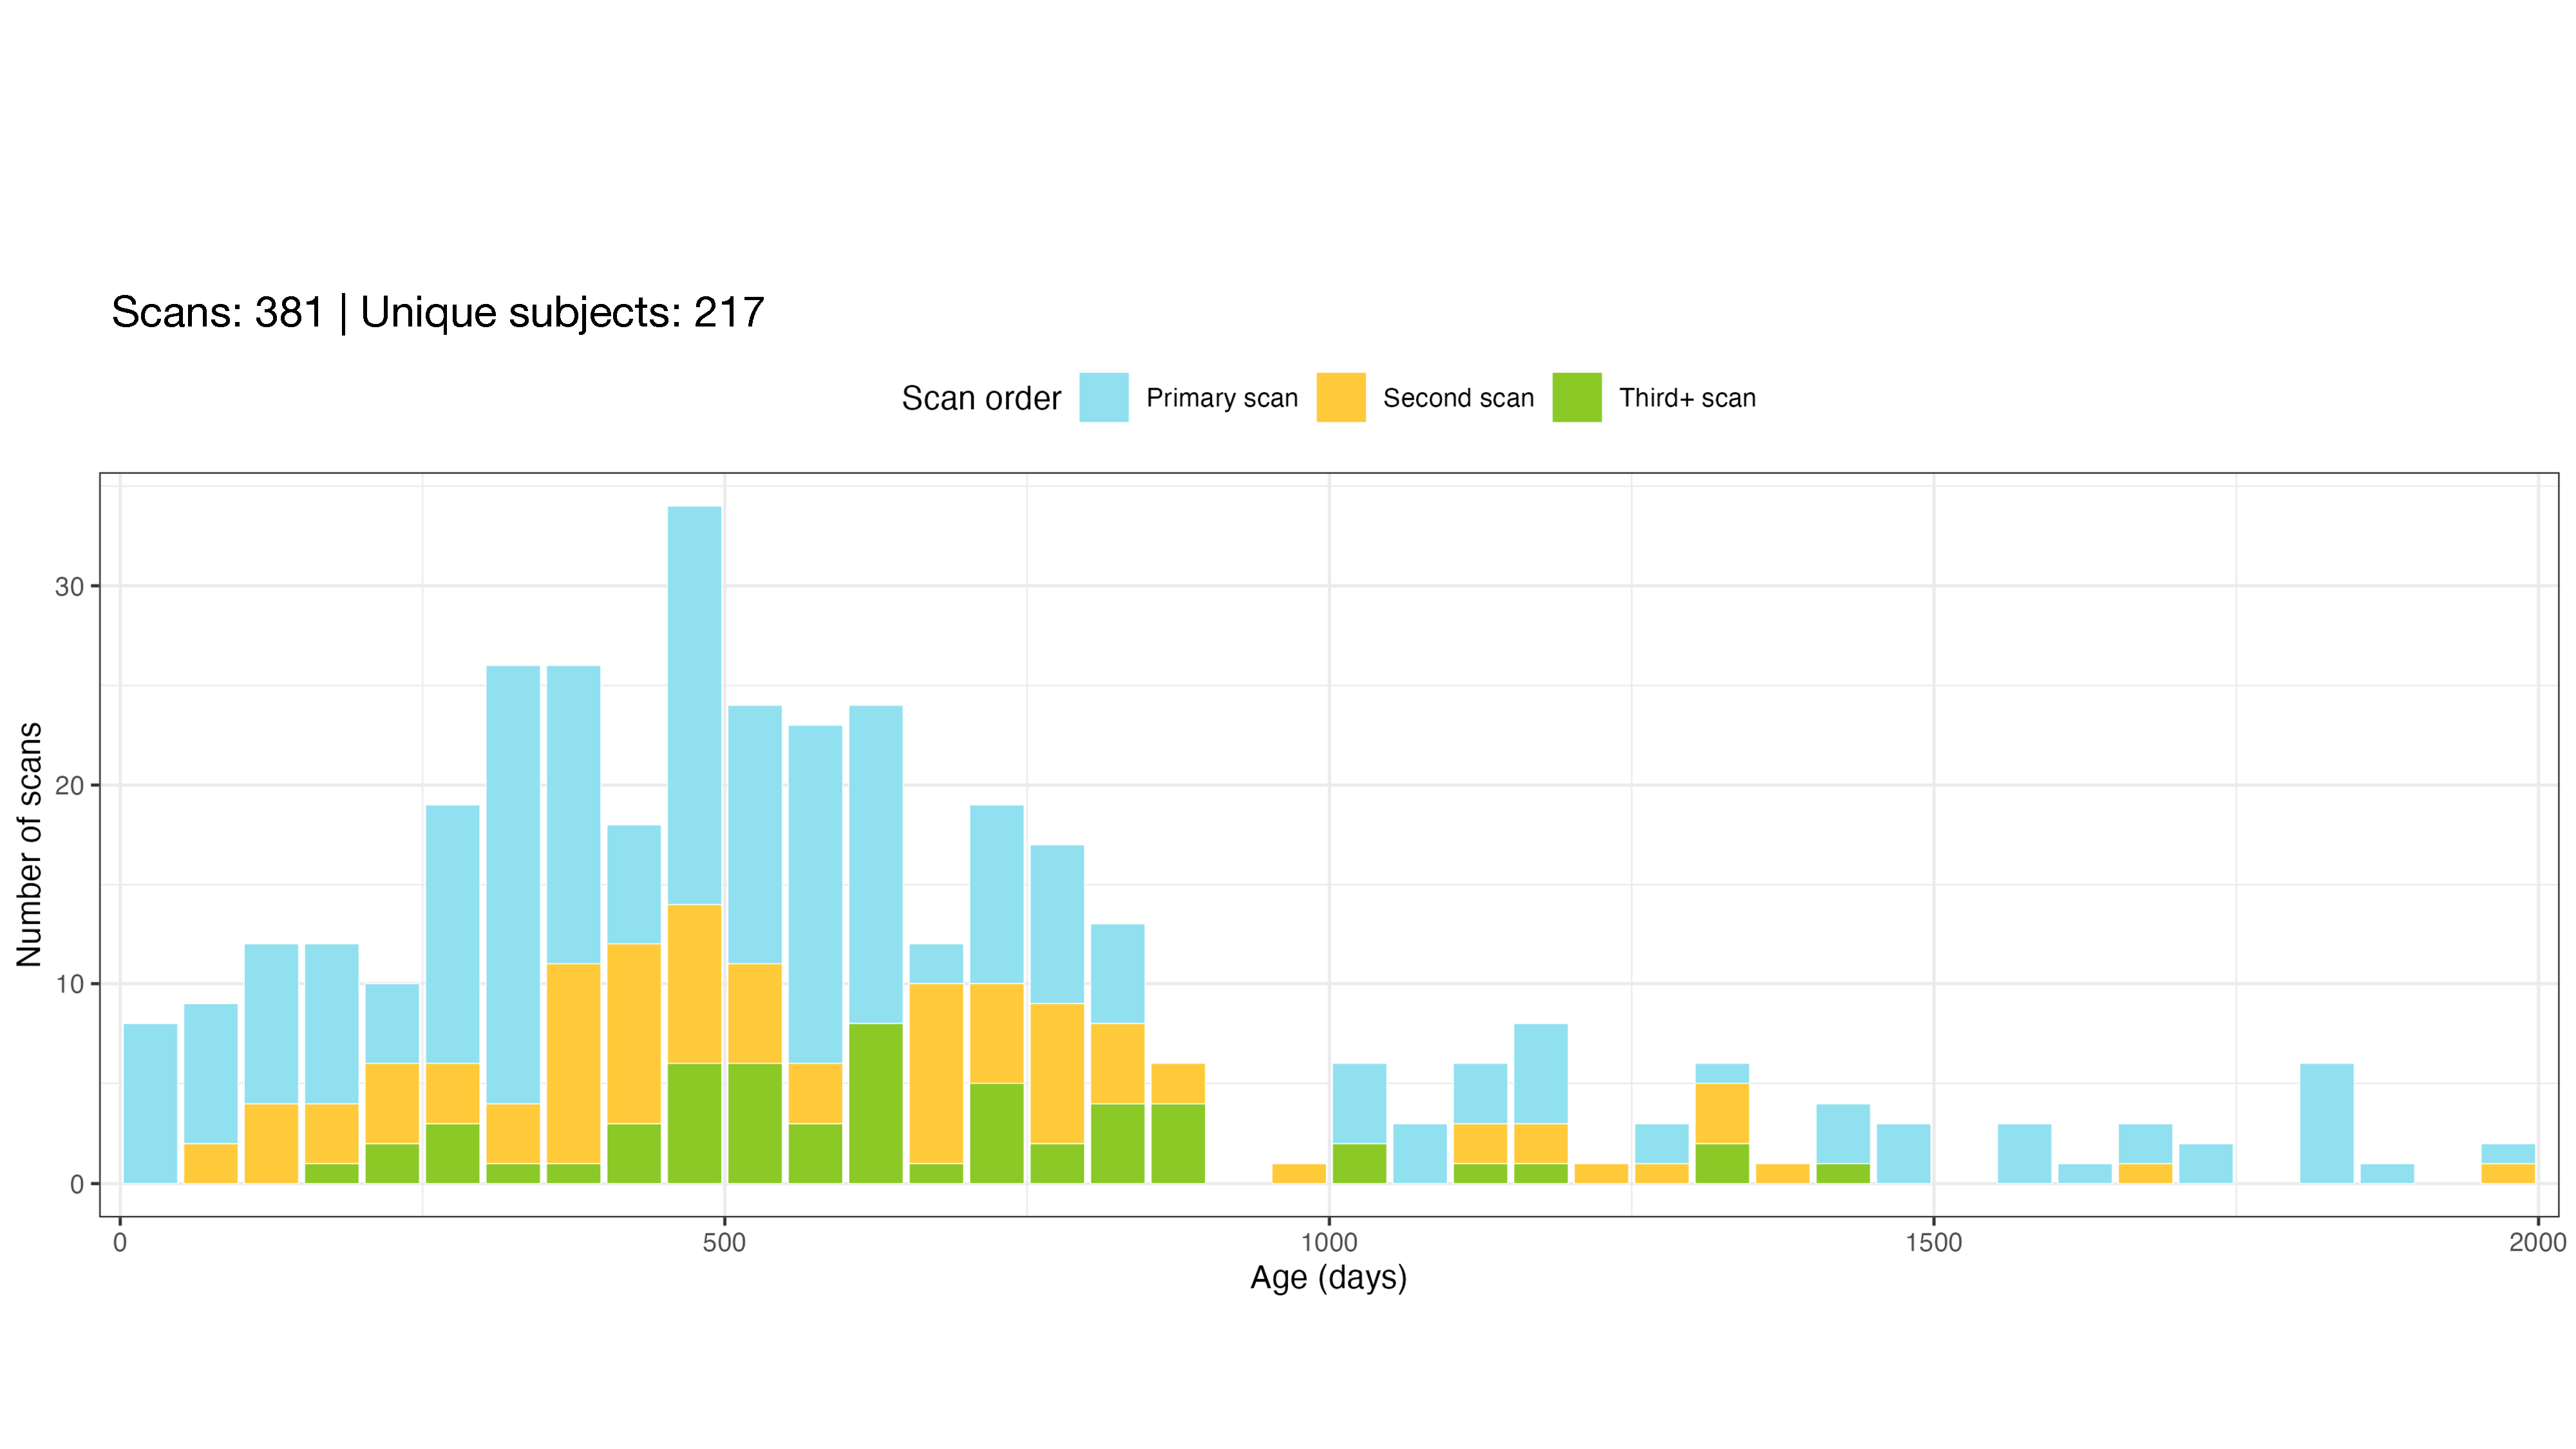
\includegraphics[width=0.95\linewidth]{figure/Figure1_population.pdf}
  \caption{\textbf{$|$ Population age distribution and sample composition.}
  Histogram bars show the distribution of matched scan ages (in days) across the early-childhood window analyzed in this study. Stacked colors indicate scan order within participant: first scan (blue), second scan (yellow), and third-or-later scan (green). We show three bin-width resolutions (20, 50, and 100 days) to illustrate both fine-grained and coarse-grained sampling density across age.}
  \label{fig:supplementary_population}
\end{figure}

\subsection{Denoising}\label{subsec:denoising}
Resting-state fMRI data from three healthy participants were obtained from the ON-Harmony dataset\cite{warringtonResourceDevelopmentComparison2023}. Data were acquired using a 3T Philips Achieva scanner with a repetition time of 1150\,ms (400 timepoints) and 2.4\,mm isotropic resolution. We compared our method, OS-SVD\cite{huynhOptimalShrinkageDenoising2024}, with two state-of-the-art techniques: MP-PCA\cite{veraartDiffusionMRINoise2016} and NORDIC\cite{vizioliLoweringThermalNoise2021}.
This denoising and individual-gradient evaluation framework follows our prior work on precision functional gradients and optimal-shrinkage fMRI denoising\cite{maoPrecisionFunctionalGradients2026,maoLoweringThermalNoise2024}.

\textbf{OS-SVD.} OS-SVD aggregates the time series of a group of neighboring voxels into a 2D matrix. It then applies singular value decomposition (SVD) followed by optimal shrinkage (OS) to separate signal and noise components.

\textbf{MP-PCA.} MP-PCA calculates the covariance matrix of the 2D signal matrix and uses Marcenko-Pastur (MP) curve-fitting to separate signal and noise components.

\textbf{NORDIC.} NORDIC uses MP-PCA as its core denoising algorithm, but incorporates g-factor information for performance improvement.

Denoising performance was assessed using temporal signal-to-noise ratio (tSNR) and residual maps. We compared these denoising methods directly under matched preprocessing settings.
\begin{figure}[t]
  \centering
  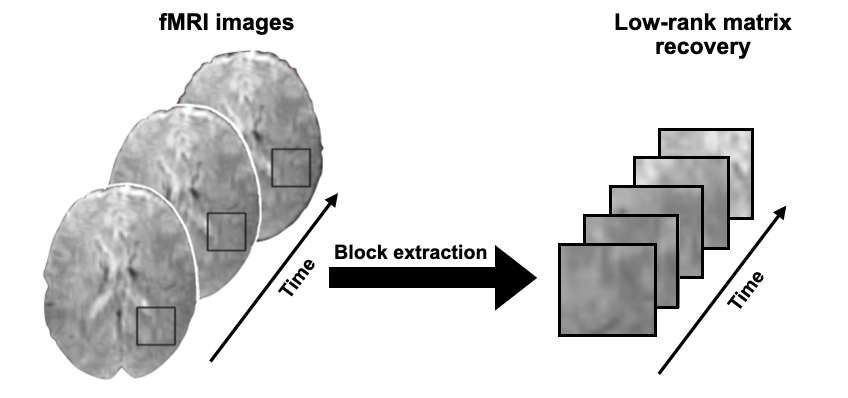
\includegraphics[width=0.95\linewidth]{figure/Figure2_denoising.png}
  \caption{\textbf{$|$ Denoising workflow.}}
  \label{fig:denoising_method}
\end{figure}

\subsection{Connectivity matrix construction}
\noindent\underline{Structural connectivity matrix}\label{subsec:SC} \hfill\\
% here there's an hdot between d1, d2 and dk is it supposed to be a value? 
Edge weights $A_{ij}$ connecting each pair of nodes in the adjacency matrix $A$ of each brain network were computed from the streamlines as follows. Each endpoint of a streamline can be associated with $K$ candidate vertices. Denoting the distances of the endpoint to the vertices as $0 \leq d_{1} \leq d_{2} \leq \hdots \leq d_{K}$, the connection weight for the $i$-th vertex can be defined as 
\begin{equation}
    w_{i} = \frac{\frac{1}{d_{i}}}{\sum_{k=1}^{K}\frac{1}{d_{k}}}.
\end{equation}
To avoid numerical complication when $d_{1} = 0$, we define $h_{i} = d_{1}/d_{i}$ with $h_{1} = 1$ and therefore
\begin{equation}
    w_{i} = \frac{h_{i}}{\sum_{k=1}^{K}h_{k}}.
\end{equation}
Considering two endpoints of a streamline, denoted with 1 and 2, the connection weight between vertices $i$ and $j$ is
\begin{equation}
    w_{ij} = w_{i}^{1}w_{j}^{2}.
\end{equation}
Note that $\sum_{i,j}w_{ij}=1$.
Streamlines causing self connections ($w_{ij}>0$ for $i=j$) are considered invalid and are excluded.
To account for regional size differences, streamline counts were normalized by the sum of the cortical volumes of the connected regions, yielding a matrix that reflects the relative strength of white matter connectivity between all region pairs. Finally, each subject's SC matrix was $z$-normalized. 

\noindent\underline{Functional connectivity matrix}\label{subsec:FC} \hfill\\
For each subject and scan, preprocessed resting-state fMRI data were projected onto the cortical surface, yielding vertex-wise time series for the left and right hemispheres (each \(10{,}242 \times 420\) vertices~\(\times\)~timepoints). Vertices containing zero or NaN values were excluded prior to analysis. Functional connectivity (FC) was computed within each temporal segment by calculating the Pearson correlation coefficient between the time series of all vertex pairs, resulting in a vertex-by-vertex correlation matrix. To enhance network specificity and reduce spurious connections, each vertex’s FC profile was sparsified by retaining only the strongest 10\% of correlations per row and setting the remaining values to zero. We then computed a profile-similarity kernel across vertices by treating each vertex's thresholded FC pattern as a feature vector and calculating pairwise cosine similarity between all vertices. The resulting similarity values were converted to a normalized angular kernel within the range \([0,1]\) according to  
\[
K = 1 - \frac{\arccos(\text{cosine similarity})}{\pi}.
\]
This kernel quantifies the degree of functional similarity between vertices, where higher values indicate more similar connectivity profiles. The resulting kernel matrices were inserted back into the full cortical surface space (left and right hemispheres combined; \(20{,}484 \times 20{,}484\)) and saved for subsequent analyses.

\subsection{Functional gradients}\label{subsec:functional_gradients}
Following the functional-gradient workflow described in prior work\cite{taylorFunctionalHierarchyHuman2024}, we computed subject-level cortical gradients from thresholded functional connectivity matrices. For each acquisition, vertex-wise FC was defined by Pearson correlation between BOLD time series:
\[
\mathrm{FC}_{ij}=\mathrm{corr}\!\left(x_i(t),x_j(t)\right), \quad i,j\in\{1,\dots,20484\}.
\]
For each subject, FC matrices were averaged across acquisitions, then row-wise sparsified by retaining the strongest 10\% of connections per row. We next computed profile similarity between thresholded FC profiles using cosine similarity and converted it to a normalized-angle affinity kernel:
\[
\cos_{ij}=\frac{f_i^\top f_j}{\|f_i\|\,\|f_j\|}, \qquad
K_{ij}=1-\frac{\arccos(\cos_{ij})}{\pi}, \quad K_{ij}\in[0,1],
\]
where \(f_i\) is the thresholded FC profile of vertex \(i\). Diffusion-map embedding (BrainSpace implementation) was applied to this affinity matrix. Let \(D\) be the degree matrix with \(D_{ii}=\sum_j K_{ij}\); the row-stochastic operator is
\[
P=D^{-1}K,
\]
and gradients were obtained from its leading non-trivial eigenvectors:
\[
P\psi_m=\lambda_m\psi_m, \qquad m=1,\dots,k.
\]
We extracted the first 10 gradients per subject and aligned them to a template gradient basis by one-shot orthogonal Procrustes (without scaling or mean-centering). Denoting subject and template gradients by \(X,Y\in\mathbb{R}^{N\times 10}\), we solved
\[
R^*=\arg\min_{R}\|XR-Y\|_F^2,\qquad \text{s.t. } R^\top R=I.
\]
Using \(M=X^\top Y=U\Sigma V^\top\), the optimal transform is
\[
R^*=UV^\top,\qquad X_{\text{aligned}}=XR^*.
\]
After alignment, each gradient sign was checked against the template and flipped when needed to preserve correspondence across subjects.

\begin{figure}[t]
  \centering
  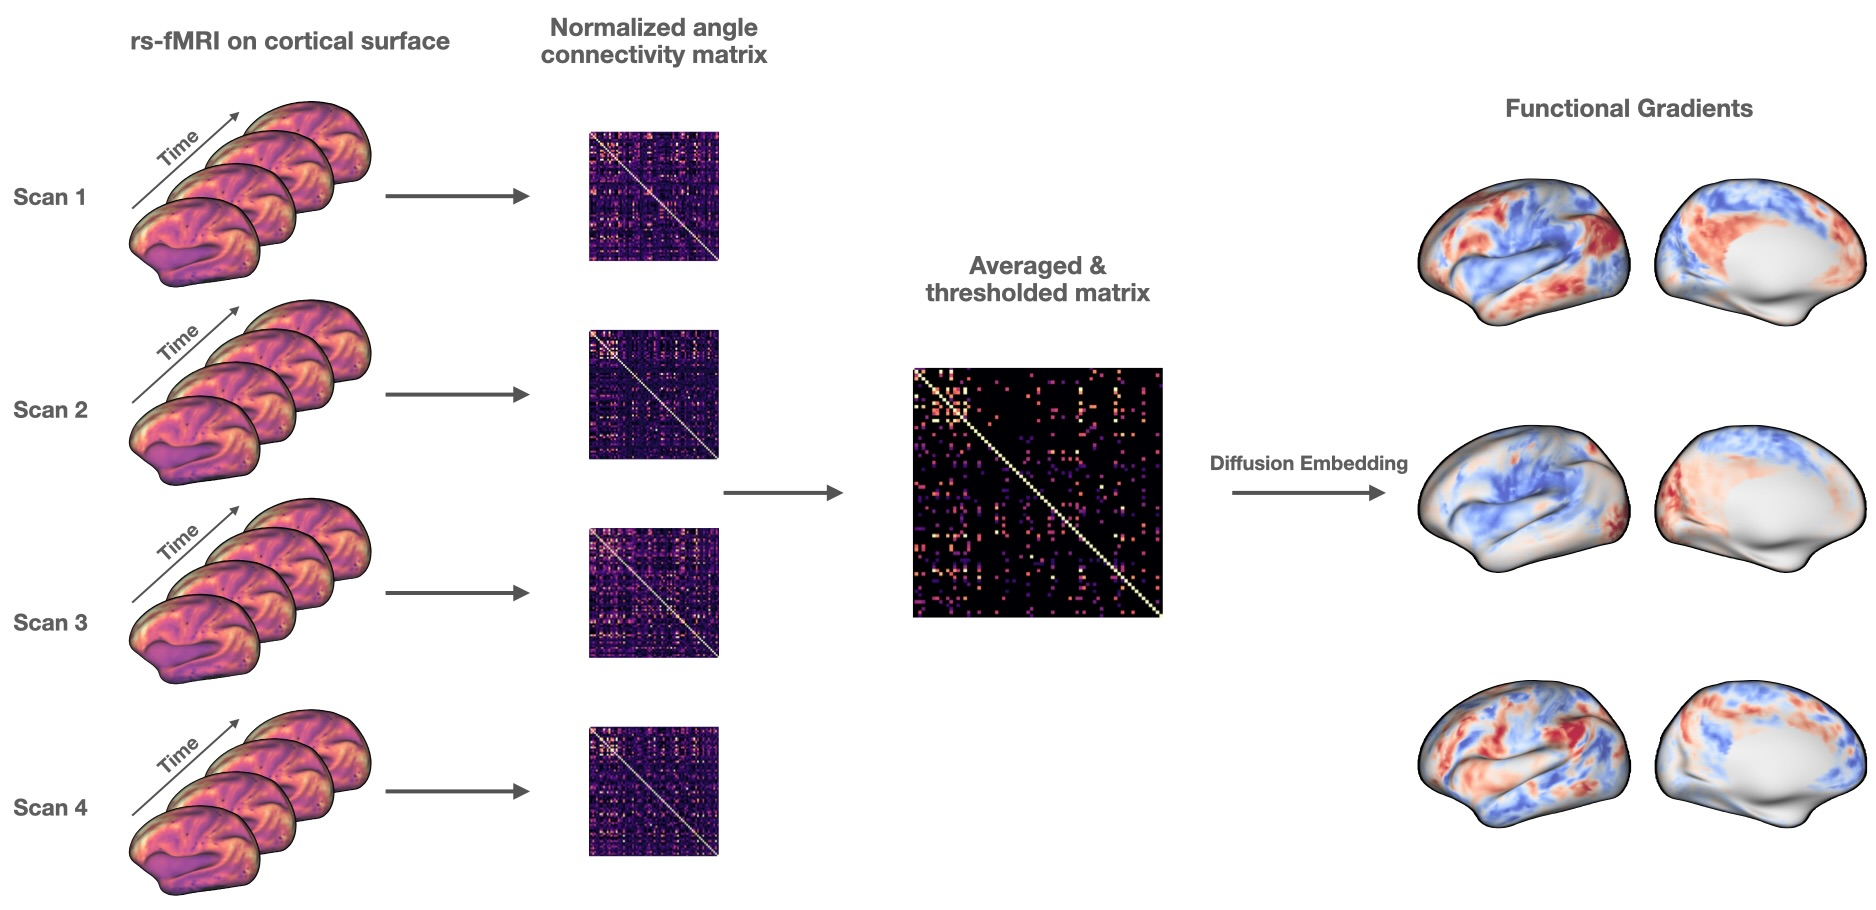
\includegraphics[width=0.95\linewidth]{figure/Figure3_individualgradients.jpeg}
  \caption{\textbf{$|$ Individual functional gradients and template alignment.}
  Subject-level cortical gradients were derived from thresholded FC profile similarity using diffusion-map embedding and aligned to the template basis using one-shot orthogonal Procrustes transformation.}
  \label{fig:individual_gradients}
\end{figure}

\clearpage
\subsection{Structure-Function Coupling (SFC)}\label{subsec:SFC}
SFC is calculated as the Pearson correlation between structural connectivity and functional connectivity profiles of each vertex. We calculated the Pearson correlation coefficient between these two profiles, resulting in a single SFC value for each vertex. This process was repeated for all vertices on the cortical surface, yielding a vertex-wise map of SFC for each subject. 
To quantify how much SFC fluctuates around its mean over time, we also computed a temporal SFC variance measure. 
Instead of estimating a single ``static'' SFC value per region, as in our primary analyses, we first divided each BCP scan (420 volumes) into 10 non-overlapping, temporally contiguous windows and computed a separate functional connectivity matrix for each window using the procedure described in the ``Functional Connectivity'' section. 
For each subject and each vertex, we then computed an SFC value within each window by relating that vertex's window-specific functional connectivity profile to its corresponding structural connectivity profile (excluding self-connections and entries in which either structural or functional connectivity was zero). 
This yielded 10 SFC values per vertex per subject. 
A vertex's temporal SFC variance was defined as the variance of these 10 time-resolved SFC estimates. 
Together with the static SFC metric (overall strength of structure--function coupling), this temporal SFC variance index captures how strongly a region's coupling to its structural backbone fluctuates over the course of the resting-state scan.

\begin{figure}[t]
  \centering
  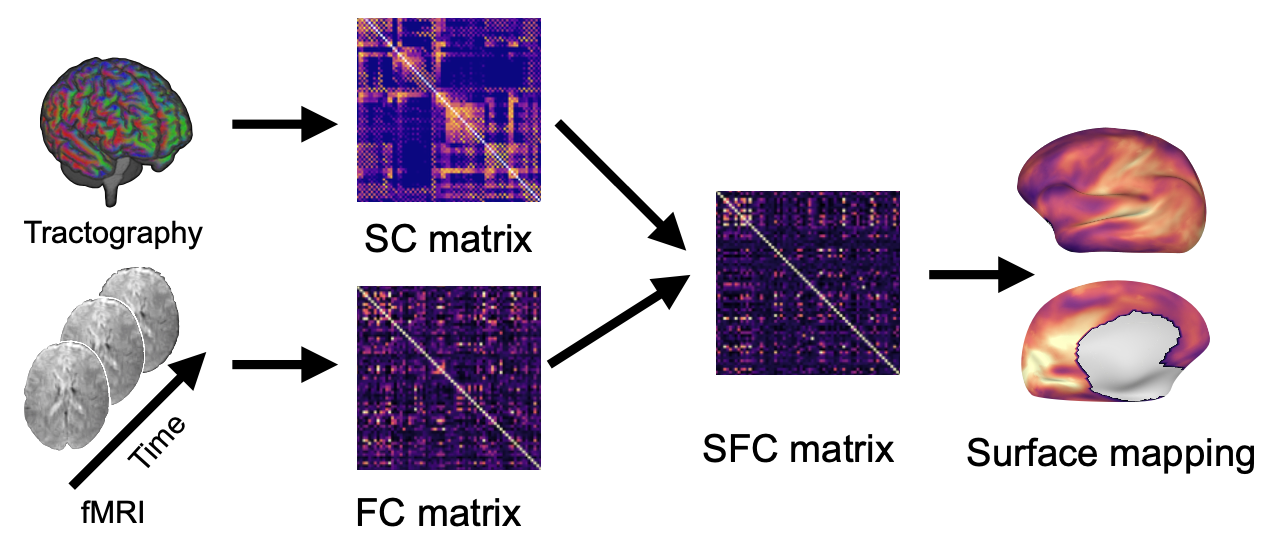
\includegraphics[width=0.95\linewidth]{figure/Figure4_SFCmethod.png}
  \caption{\textbf{$|$ Structure-function coupling (SFC) computation workflow.}
  Vertex-wise SFC was computed as the Pearson correlation between each vertex's structural and functional connectivity profiles, with additional time-windowed estimation used to derive temporal SFC variance.}
  \label{fig:sfc_method}
\end{figure}

\subsection{Excitation-inhibition balance}
Previous modeling work has shown that shifts in the excitation–inhibition ratio (E/I ratio) are reflected in the spectral properties of neural activity, in particular in the exponent of the 1/f power-law component, which is mathematically related to the Hurst exponent of the signal time series\cite{trakoshisIntrinsicExcitationinhibitionImbalance2020,bruiningMeasurementExcitationinhibitionRatio2020,gaoInferringSynapticExcitation2017}. This relationship has been validated both in simulated functional data and in mouse resting-state fMRI during chemogenetic modulation of pyramidal cell excitability, where an increased E/I ratio corresponds to a decrease in the Hurst exponent\cite{gaoInferringSynapticExcitation2017}.

We projected each subject's preprocessed resting-state fMRI data onto the cortical surface and obtained time series for 20,484 vertices (10,242 per hemisphere). The Hurst exponent was estimated from each vertex’s BOLD time series using a univariate maximum-likelihood framework in combination with a discrete wavelet transform. For each subject and vertex, we first estimated the power spectral density (PSD) by taking the median of the squared magnitude of the sliding-window short-time Fourier transform (STFT). We used the median rather than the mean (as in Welch's method) to better accommodate the non-Gaussian distribution of spectral estimates and to reduce the impact of extreme outliers\cite{gaoInferringSynapticExcitation2017}. To obtain the 1/f power-law exponent (log-log slope), we then fit a robust linear regression to the log-transformed PSD across the specified frequency band (30-50 Hz) and took the slope of this fit as the 1/f exponent\cite{gaoInferringSynapticExcitation2017}.

\begin{figure}[t]
  \centering
  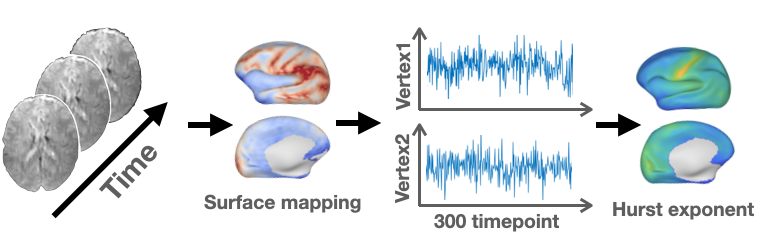
\includegraphics[width=0.95\linewidth]{figure/Figure5_hurstmethod.png}
  \caption{\textbf{$|$ Excitation-inhibition balance (Hurst) estimation workflow.}
  The Hurst exponent was estimated from vertex-wise rs-fMRI time series to index E/I-related dynamics across the cortex.}
  \label{fig:hurst_method}
\end{figure}

\subsection{Myelination calculation}\label{subsec:myeliation}
%i once have one sentence under fMRI preprocessing talk about it, can you pls check if this is true? 
Intracortical myelination was estimated using the T1w/T2w ratio, which has been shown to correlate with histological measures of myelin content\cite{glasserMappingHumanCortical2011}. For each subject, we computed the T1w/T2w ratio at each vertex on the cortical surface by dividing the intensity of the T1-weighted image by that of the T2-weighted image. This ratio was then normalized across subjects to account for inter-individual variability in signal intensity and to facilitate group-level analyses. The resulting vertex-wise myelin maps were used in subsequent analyses to examine their relationship with SFC and other developmental metrics.

\begin{figure}[t]
  \centering
  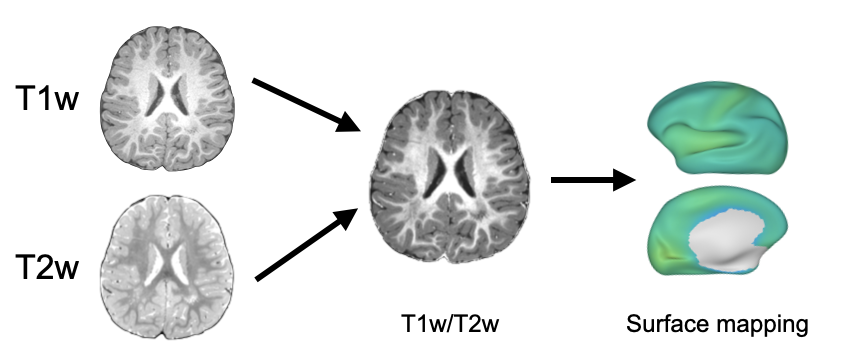
\includegraphics[width=0.95\linewidth]{figure/Figure6_myelinationmethod.png}
  \caption{\textbf{$|$ Intracortical myelination (T1w/T2w) computation workflow.}
  Vertex-wise T1w/T2w ratios were derived on the cortical surface to estimate intracortical myelin and used for downstream developmental analyses.}
  \label{fig:myelin_method}
\end{figure}

\subsection{Correlation calculation}\label{subsec:correlation}
\subsubsection{Spatial correlation}
For each timepoint $t$, we assembled two spatial maps across vertices: $X_t(v)$ (SFC) and $Y_t(v)$ (myelination or Hurst).  
We computed the Pearson correlation
\[
r_t = \mathrm{corr}\big(X_t(v), Y_t(v)\big)
\]
across $v = 1,\dots,10242$, with a two-sided p-value.  
This produced 401 spatial correlations per pairing (SFC-myelination and SFC-Hurst).  
Timepoints with $p < 0.001$ were considered significant. See more in \nameref{subsec:GAMM}.

\subsubsection{Temporal correlation}
For each subject-age timepoint (401 total), we derived vertex-wise maps on the fsaverage surface (10,242 vertices) for: (i) structure–function coupling (SFC), (ii) intracortical myelination (T1w/T2w ratio), and (iii) the Hurst exponent (functional time-series scaling).
For each vertex $v \in \{1,\dots,10242\}$, we formed two developmental trajectories across timepoints $t = 1,\dots,401$:  
$X_v(t)$ (SFC) and $Y_v(t)$ (either myelination or Hurst).  
We computed the Pearson correlation
\[
r_v = \mathrm{corr}\big(X_v(t), Y_v(t)\big)
\]
and its two-sided p-value. Vertices were considered significant at $p < 0.001$.  
This procedure was performed twice: (1) SFC–myelination and (2) SFC-Hurst, yielding two vertex-wise correlation maps.

\subsubsection{p-spin analysis}
To account for spatial autocorrelation on the cortical surface, we additionally performed a permutation spin test (p-spin) for each spatial-correlation analysis. In this framework, \(X\) was fixed as the vertex-wise SFC map and \(Y\) was the vertex-wise myelination map or Hurst map. We generated 1,000 spherical rotations of \(Y\) (within hemisphere), recomputed the correlation after each rotation, and built a null distribution \(\{r_t^{\mathrm{spin}}\}\). Two-sided spin-based significance was computed as
\[
p_{\mathrm{spin}}=\frac{1+\sum_{b=1}^{B}\mathbf{1}\!\left(|r_{t,b}^{\mathrm{spin}}|\ge |r_t|\right)}{1+B},
\]
with \(B=1000\). We report \(r_t\) together with \(p_{\mathrm{spin}}\) for both pairings (\(X=\) SFC, \(Y=\) myelination or Hurst).

\subsubsection{Mediation analysis}\label{subsec:mediation_pathway}
To complement vertex-wise correlation analyses, we performed scan-level pathway analyses to test whether microstructural and dynamical pathways explained SFC variation. For each scan, we derived one summary value per modality: mean SFC, mean Hurst exponent, mean T1w/T2w myelin, mean FC, and mean SC. For SFC, Hurst, and myelin, we first computed hemisphere-specific means and then averaged left and right hemispheres. SC and FC were reconstructed from part-wise 400-ROI files and aggregated to one scan-level mean connectivity value per modality.  

To align modalities across acquisitions, we anchored matching on SFC scans and matched the nearest same-subject scan from each other modality within a 30-day tolerance. For myelin, age values were converted from months to days using $\mathrm{Age}_{\mathrm{days}} = \mathrm{Age}_{\mathrm{months}} \times 30.5$ prior to matching.  

All pathway models were fit as linear mixed-effects models with subject-specific random intercepts to account for repeated longitudinal observations:
\[
Y_{ij} = \beta_0 + \beta_1 X_{ij} + (1 \mid \mathrm{ID}_i) + \epsilon_{ij},
\]
where $X_{ij}$ is the pathway predictor for subject $i$ at scan $j$, and covariates were held fixed across path equations within each model.
Model fitting and mediation workflows were implemented in R using broadly useful utilities from the \texttt{bruceR} package \cite{bao2021bruceR}.

\textbf{Direct pathway model.}  
For instance, for myelin $\rightarrow$ SFC fit:
\[
\mathrm{SFC}_{ij} = \gamma_0 + bM_{ij} + (1 \mid \mathrm{ID}_i) + \eta_{ij},
\]
where $M_{ij}$ denotes intracortical myelin.

\textbf{Serial mediation models.}  
For myelin $\rightarrow$ SC $\rightarrow$ SFC, we fit:
\[
\mathrm{SC}_{ij} = \delta_0 + d_{21}M_{ij} + (1 \mid \mathrm{ID}_i) + \epsilon_{2,ij},
\]
\[
\mathrm{SFC}_{ij} = \gamma_0 + b_1M_{ij} + b_2\mathrm{SC}_{ij} + (1 \mid \mathrm{ID}_i) + \eta_{ij}.
\]
For this model, the serial indirect effect is:
\[
IE_{\mathrm{serial}} = d_{21}b_2.
\]
The direct and total effects of myelin on SFC are:
\[
b_{\mathrm{direct}} = b_1,\qquad
b_{\mathrm{total}} = b_1 + d_{21}b_2.
\]

\textbf{Age-dependent mediation extension.}
To allow pathway strengths to vary developmentally, we additionally expressed path
coefficients as age-dependent functions:
\[
\mathrm{SC} = d_{21}(t)M + \epsilon_2,\quad
\mathrm{SFC} = b_1(t)M + b_2(t)\mathrm{SC} + \epsilon_Y.
\]
Age-specific serial indirect effects were defined as:
\[
IE_{\mathrm{serial}}(t)=d_{21}(t)b_2(t).
\]
For summary, we report peak serial mediation magnitude and its timing:
\[
IE_{\max}=\max_t |IE_{\mathrm{serial}}(t)|,\qquad
t^*=\arg\max_t |IE_{\mathrm{serial}}(t)|.
\]
Because averaging age-specific indirect effects is a different estimand from the
age-independent serial indirect effect, we prioritize trajectory-level summaries over a
single global mean effect.

\textbf{Integrated dual-channel model.}  
We additionally fit a piecewise integrated model combining structural and dynamics channels:
myelin $\rightarrow$ SC $\rightarrow$ SFC and Hurst $\rightarrow$ FC $\rightarrow$ SFC, with direct myelin $\rightarrow$ SFC and Hurst $\rightarrow$ SFC paths in the final outcome equation. Channel-specific and total indirect effects were computed as products/sums of fitted path coefficients.

Uncertainty for direct and indirect effects was estimated using subject-level bootstrap resampling (2,000 replicates), with 95\% percentile confidence intervals. For indirect effects, two-sided bootstrap p-values were computed from the smaller tail proportion relative to zero. For models containing multiple indirect pathways (e.g., integrated dual-channel models), multiplicity across indirect effects was controlled at $\alpha_{\mathrm{FWER}}=0.05$ using Holm correction (Bonferroni shown as reference). We also tracked the number of bootstrap replicates showing singular mixed-model fits as a model-stability diagnostic.

\subsubsection{Generalized Additive Mixed Modeling}\label{subsec:GAMM}
We used Generalized Additive Mixed Model (GAMM) curve fitting to model nonlinear changes of each brain feature over a time window of 0 to 5 years. To capture rapid developmental changes in the early postnatal stage, we applied a log transformation to the age variable.
For each vertex, we modeled changes $y$ as a function of age $t$ (fixed effect), individual $s$ (random effect) to account for longitudinal scans. The model incorporated smooth nonlinear functions $s_{\cdot}$, intercept $\beta$, and error $\epsilon \in \mathcal{N}(0,\sigma^2)$: $y=f(t,s)=\beta + s_t(\log_2(t+1) + s_s(s) + \epsilon$ with $t$ in years.
We set $s_{\cdot}$ to be cubic regression splines and used restricted maximum likelihood (REML) for smoothing parameter estimation, following \cite{taylorFunctionalHierarchyHuman2024}.
The BCP dataset was acquired at two imaging sites: the University of North Carolina at Chapel Hill (UNC) and the University of Minnesota (UMN). However, we found no significant differences in data distribution, microstructural values, or cortical gradients between sites. Therefore, site effects were not included in our model. 

\noindent\underline{Age effect}
To assess the influence of age, we contrasted the explanatory power of a full model, which included a smooth term for log-transformed age, with that of a reduced model without age. 
We defined the age effect as the change in adjusted $R^2$ ($\Delta R_{\text{adj}}^2$) between the full and reduced models, such that $\Delta R_{\text{adj}}^2$ indexes the variance uniquely attributable to age\cite{luoTwoAxesWhite2026}.


\section{Results}

% decide i dont need overview  \subsection{Overview}
% To delineate the development of structure--function coupling (SFC) from birth to age five, we analyzed multimodal MRI data from the Baby Connectome Project ($N= [Insert N]$, age 0--5 years)\cite{howellUNCUMNBaby2019}. We defined vertex-wise SFC as the Pearson correlation between a region's structural connectivity (SC) strength and its functional connectivity (FC) profile (Methods).

% We first characterized global developmental trends. Averaged across the cortex, SFC, intracortical myelination (T1w/T2w ratio), and excitation--inhibition balance (indexed by the Hurst exponent, $H$) all exhibited robust age-related changes (Fig.~\ref{fig:timeline}a). From birth to five years, mean SFC increased by approximately 23\%, indicating a progressive alignment of functional signals with underlying structural architecture. Concurrently, intracortical myelin increased by $\sim$15\%, while the Hurst exponent decreased by $\sim$6\%, reflecting a global shift toward higher excitation--inhibition (E/I) ratios and faster neural dynamics. These trajectories persisted after controlling for sex, motion, and site effects (Fig.~\ref{fig:timeline}b), establishing that early childhood is defined by three concurrent macro-scale trends: strengthening structure--function alignment, microstructural maturation, and the remodeling of cortical temporal dynamics.

\subsection{OSSVD improve performance of fMRI and individual gradient}
% Placeholder: denoising result details will be added later.
\begin{figure}[t]
  \centering
  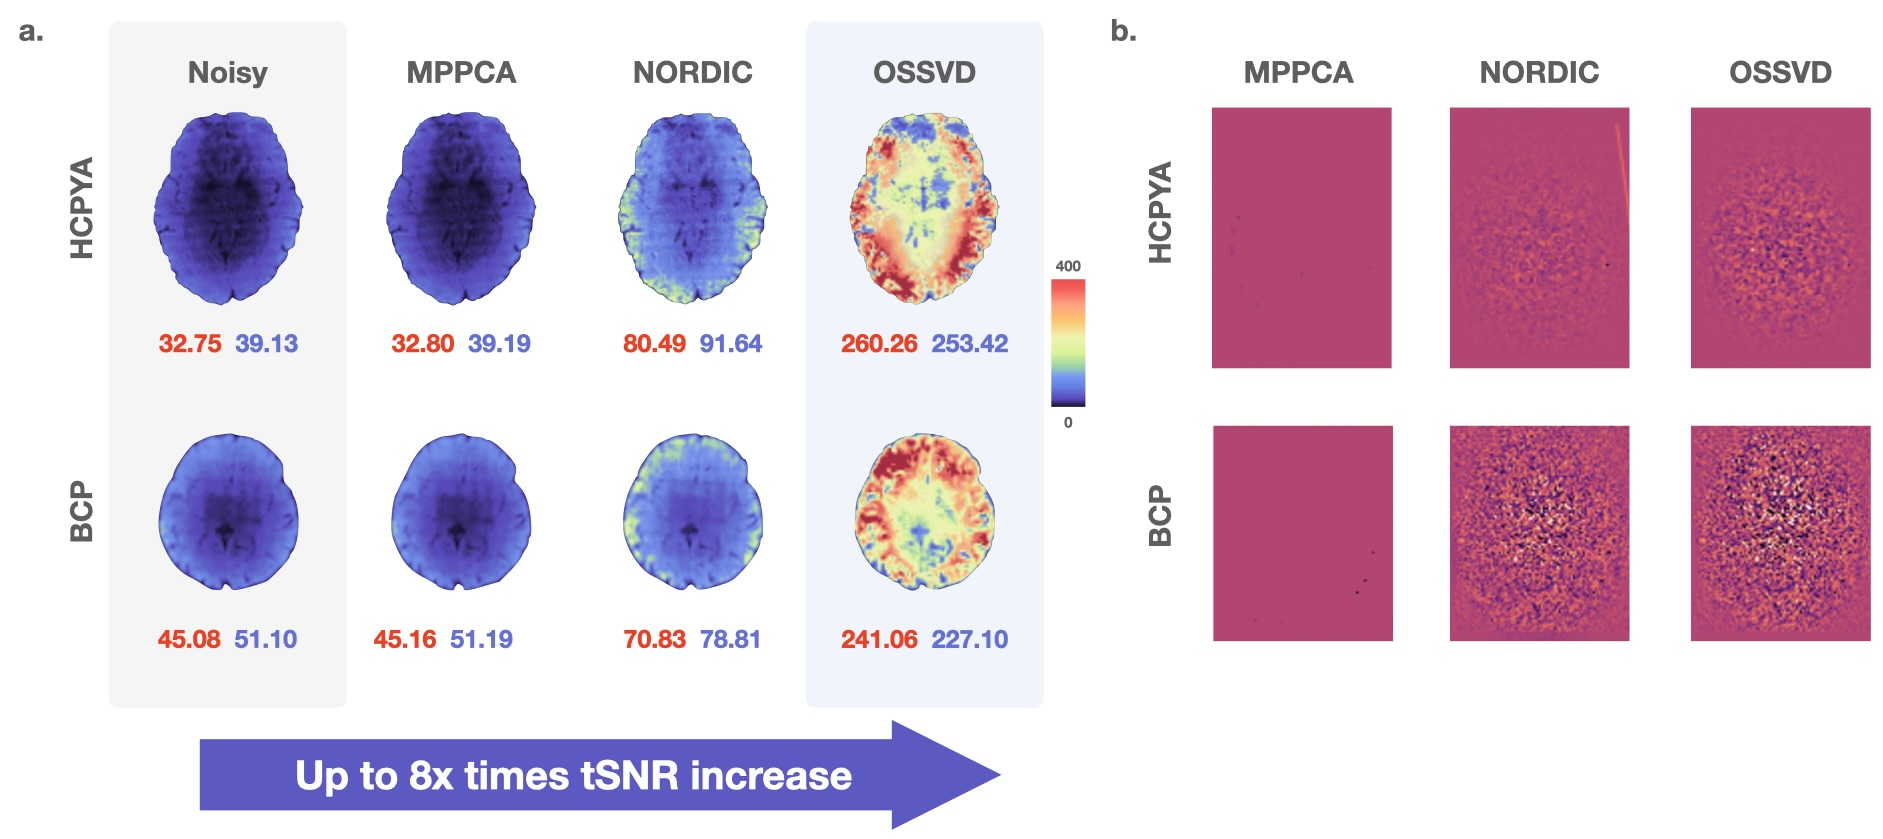
\includegraphics[width=0.95\linewidth]{figure/Figure7_denoisingresult.jpeg}
  \caption{\textbf{$|$ Effects of noise removal.} (a) Temporal signal-to-noise ratio (tSNR) before and after denoising. OS-SVD achieves the largest tSNR improvement, particularly in gray matter, and outperforms MP-PCA and NORDIC. (b) Residual maps show no discernible loss of structural information after denoising.}
  \label{fig:denoising_result}
\end{figure}

\begin{figure}[t]
  \centering
  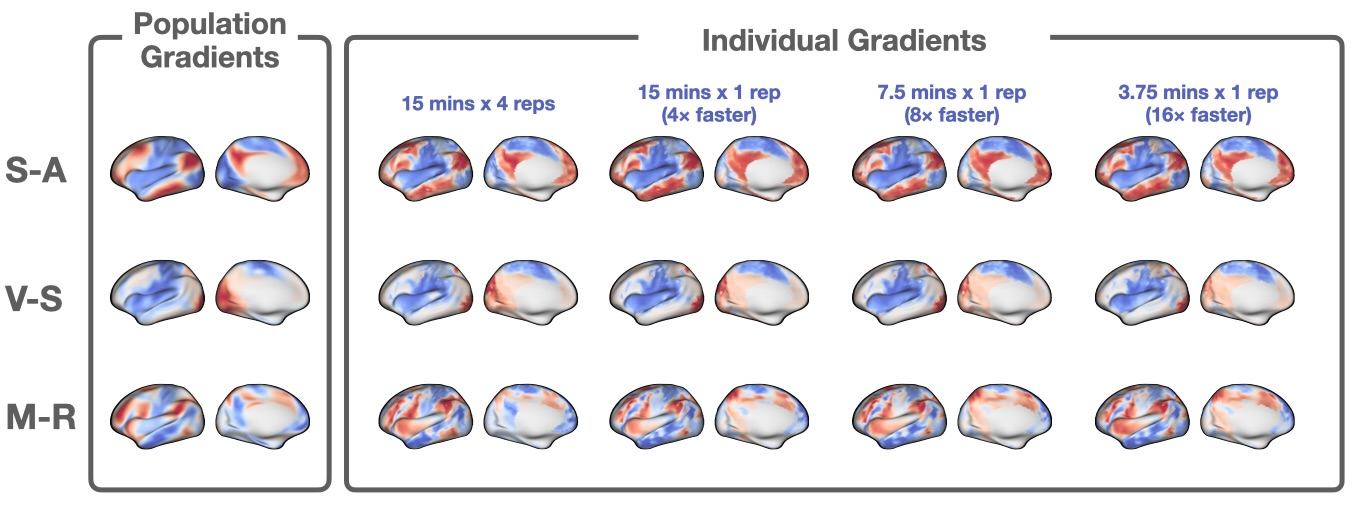
\includegraphics[width=0.95\linewidth]{figure/Figure8_gradientcomparison.jpeg}
  \caption{\textbf{$|$ Effects of using fewer volumes and repetitions on gradients.}
  OS-SVD preserves gradient patterns even with less than 4 minutes of data, reducing acquisition time by 16 times.}
  \label{fig:denoising_gradient_comparison}
\end{figure}

Denoising efficiency and structural preservation: OS-SVD denoising increases temporal SNR by 8 times, particularly in gray matter, significantly outperforming MP-PCA by 800\% and NORDIC by 300\% (Fig.~\ref{fig:denoising_result}a). Both OS-SVD and NORDIC produce residual maps with no discernible structural features, indicating that only noise is removed (Fig.~\ref{fig:denoising_result}b). MP-PCA yields an almost zero residual map, consistent with ineffective noise removal in this dataset.

Denoising effect on individual gradients: Denoising significantly enhances individual gradients in both adult and infant fMRI (Fig.~\ref{fig:denoising_gradient_comparison}). Without denoising, individual gradients show dispersed patterns with abrupt spatial changes, especially in higher-order gradients. OS-SVD produces smooth individual gradients, with spatial patterns that closely match the S--A (somatosensory--association), V--S (visual--sensorimotor), and M--R (modulation--representation) axes observed in population-level results.

Acceleration with temporally undersampled data: We evaluated OS-SVD's ability to produce high-quality gradients from temporally undersampled data to reduce acquisition time (Fig.~\ref{fig:denoising_gradient_comparison}). Four rs-fMRI scans per subject (1200 volumes, 15 minutes per scan, 1 hour total) were used for diffusion embedding. We then tested OS-SVD using only one scan (4x faster), with reduced volume counts of 600 (8x faster) and 300 (16x faster). With denoising, reducing volume count and scan number did not compromise gradient quality. Three principal functional connectome axes remained detectable with data acquired in under 4 minutes.

% figure 2
\subsection{Functional gradient differentiation in HBCD and BCP during early infancy}

We focused on the sensorimotor--association (S--A) gradient, which captures the primary axis of functional hierarchy from primary sensorimotor to high-order association cortices, and the visual--somatomotor (V--S) gradient, which captures a key secondary axis separating visual processing from somatomotor functions. Both functional gradients showed increasing differentiation over the first 6 months of life (Figs.~\ref{fig:gradient_timeline_bcp} and \ref{fig:gradient_timeline_hbcd}). Vertex-wise GAMMs showed divergent age-related trends at the gradient poles for both gradients, indicating that contrast between the poles increases over time. The S--A gradient showed the strongest developmental change at the primary sensorimotor pole, while the V--S gradient showed peak changes at the visual cortex pole. Association regions consistently exhibited weaker or negative effects, confirming the overall increasing gradient differentiation. These developmental patterns align with the known hierarchical organization observed in the adult brain.

To compare cross-cohort consistency, we examined gradient trajectories in both the HBCD cohort (0--6 months) and age-overlapping BCP data. The direction of change was concordant across cohorts, with early differentiation concentrated at unimodal poles and weaker change in association cortex (Figs.~\ref{fig:gradient_timeline_bcp} and \ref{fig:gradient_timeline_hbcd}), indicating that the emergence of functional hierarchy during the first postnatal months is reproducible across independent infant datasets.

\begin{figure}[t]
  \centering
  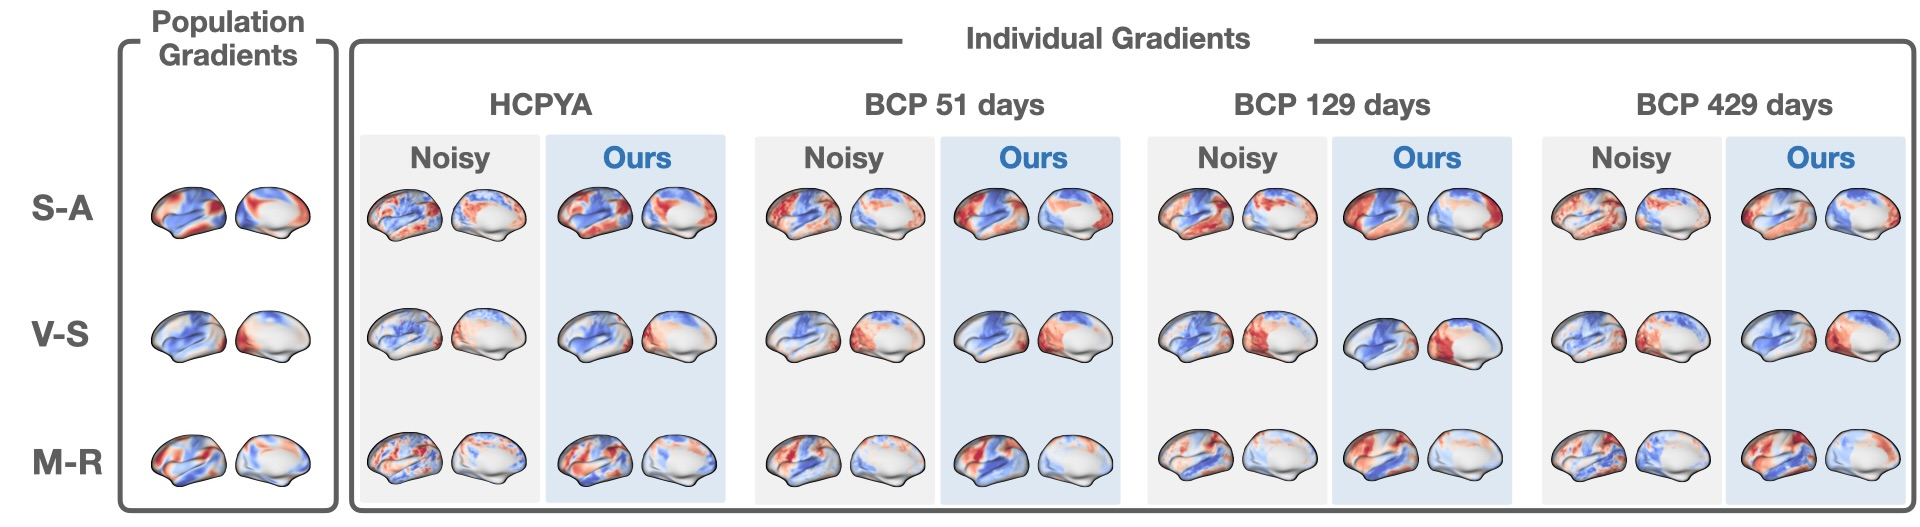
\includegraphics[width=0.95\linewidth]{figure/Figure9_gradienttimeline_BCP.jpeg}
  \caption{\textbf{$|$ Early-infant maturation of functional gradients in BCP.}
  Developmental trajectories of S--A and V--S gradients in the BCP cohort (51, 129, and 429 days) show increasing pole-to-pole differentiation, with strongest effects at primary sensorimotor and visual poles and weaker effects in association cortex.}
  \label{fig:gradient_timeline_bcp}
\end{figure}

\begin{figure}[t]
  \centering
  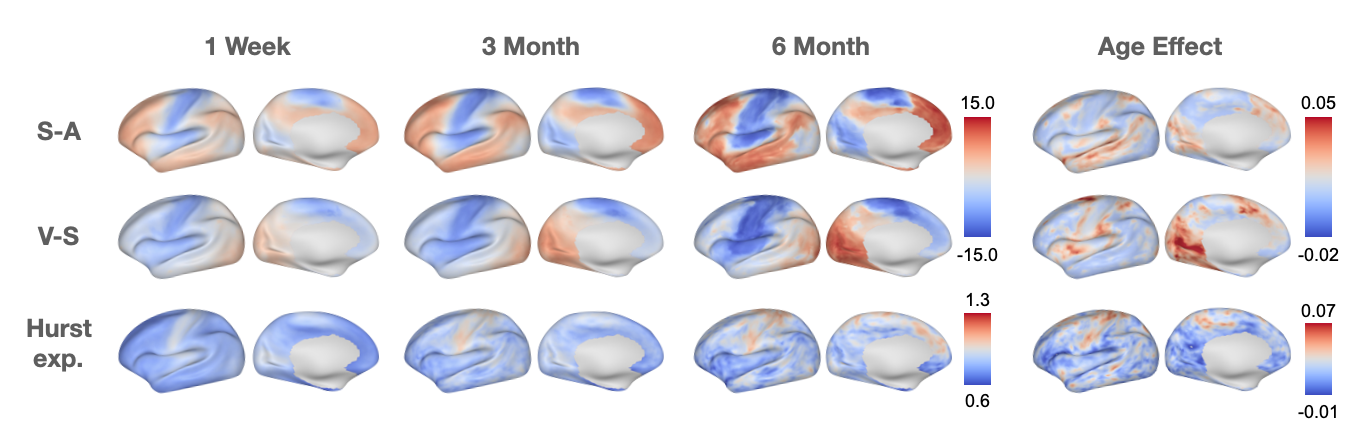
\includegraphics[width=0.95\linewidth]{figure/Figure10_gradienttimeline_HBCD.png}
  \caption{\textbf{$|$ Early-infant maturation of functional gradients in HBCD.}
  Developmental trajectories of S--A and V--S gradients during the first postnatal months show increasing pole-to-pole differentiation, with strongest effects at primary sensorimotor and visual poles and weaker effects in association cortex.}
  \label{fig:gradient_timeline_hbcd}
\end{figure}

% figure 3
\subsection{Global strengthening of structure--function coupling, myelination and temporal dynamics from birth to five years}

To characterize how structure-function coupling (SFC) and its substrates change across early childhood, we first quantified cortex-wide age trajectories for SFC, intracortical myelination, and excitation-inhibition (E/I)-related dynamics. Using multimodal MRI data from the Baby Connectome Project (BCP; $N = 221$ subjects, $372 scans$, $0$--$5$ years)\cite{howellUNCUMNBaby2019}, we computed vertex-wise SFC as the Pearson correlation between each vertex's structural connectivity (SC) and functional connectivity (FC) profiles (Methods). Intracortical myelination was indexed by the T1w/T2w ratio, and local temporal dynamics were summarized by the Hurst exponent ($H$), a scale-free measure of autocorrelation that inversely relates to the E/I ratio. Developmental change in each metric was modeled with generalized additive mixed models (GAMMs), allowing flexible nonlinear trajectories while accounting for repeated measures within individuals.

\begin{figure}[t]
  \centering
  \includegraphics[width=0.95\linewidth]{figure/Figure11_timeline.pdf}
  \caption{\textbf{$|$ Developmental trajectories of SFC, Hurst exponent, and myelination across early childhood.}
  Vertex-level cortical maps show GAMM-fitted trajectories from birth to 5 years, highlighting coordinated but regionally heterogeneous maturation of structure-function coupling, excitation-inhibition-related dynamics, and intracortical myelination.}
  \label{fig:timeline}
\end{figure}

Averaged across the cortical surface, all three measures showed pronounced age-related change from birth to five years (Fig.~\ref{fig:timeline}). Mean SFC increased by approximately $\sim\!23\%$, indicating a progressive tightening of the correspondence between functional interactions and underlying structural architecture. Over the same period, intracortical myelination increased by roughly $\sim\!15\%$, reflecting rapid maturation of the white-matter scaffold that supports long-range communication, whereas the mean Hurst exponent decreased by about $\sim\!6\%$, consistent with a global shift toward faster, more desynchronized dynamics and higher E/I ratios. These global trends remained robust after adjusting for sex, head motion and imaging site (Methods), establishing early childhood as a period of coordinated strengthening of structure--function alignment, microstructural maturation, and temporal reconfiguration.

Cortical surface maps at representative ages further revealed that these global trajectories are not spatially homogeneous (Fig.~\ref{fig:timeline}). Even in this coarse view, sensorimotor regions exhibited higher SFC and myelin and lower $H$ earlier in life, whereas association cortices showed weaker initial coupling, lower myelin, and more slowly declining $H$. These observations suggest that hierarchical differences in maturation are already apparent at the macroscale and motivate a more detailed analysis of how the sensorimotor--association axis organizes the timing and form of SFC, SC, FC, myelination and E/I development.

% \subsection{Network hierarchy constrains SFC magnitude and maturation with  structural and functional connectivity}
% Having established that structure--function coupling, myelination and temporal dynamics all change markedly from birth to five years, we next examined how this global strengthening is distributed across canonical functional networks from a vertex-wise resolution. Vertex-wise BOLD timeseries and diffusion tractography were used to construct individual $20{,}484 \times 20{,}484$ FC and SC matrices, from which we derived vertex-wise SFC and mapped it onto the cortical surface (Fig.~\ref{fig:SFC_atlas}a). The group-averaged FC and SC matrices, sorted by these networks, showed a strongly modular architecture with dense within-network and weaker between-network connectivity, particularly for unimodal VIS and SMN systems (Fig.~\ref{fig:SFC_atlas}b). Chord diagrams of FC and SC intra-network connections emphasized this organization, with strong bidirectional coupling among unimodal and attentional networks and comparatively sparser connectivity involving limbic cortex (Fig.~\ref{fig:SFC_atlas}c).
% SFC followed a rigid hierarchical organization: coupling was strongest in unimodal visual (VIS) and somatomotor (SMN) networks, intermediate in the dorsal/ventral attention (DAN/VAN) and frontoparietal (FP) networks, and weakest in the limbic (LIM) system (Fig.~\ref{fig:SFC_atlas}a). This hierarchy mirrors the underlying connectivity strengths, as violin plots of these distributions revealed that networks with high SFC also exhibited the strongest intra-network SC and FC (Extended Data Fig.~\ref{fig:supplementary_net_violin}), whereas transmodal networks with weaker internal SC/FC—especially LIM and DMN—displayed reduced SFC.
% Conversely, transmodal networks with weaker internal SC/FC—especially limbic and default mode cortex—displayed reduced SFC, consistent with greater functional flexibility and looser structural constraints. Thus, regions that are heavily wired and functionally cohesive exhibit the tightest constraints of structure on function.

% Developmental trajectories varied systematically by network. Longitudinal vertex-wise surface maps revealed that SFC increases from birth through five years across much of the cortex, with the largest age-related gains in association territories and relatively smaller changes in primary sensory and motor regions (Fig.~\ref{fig:SFC_atlas}e, top). The corresponding maps of temporal SFC variance showed decreasing variance in unimodal cortex but more heterogeneous changes in higher-order networks, suggesting early stabilization of SFC in sensory systems and prolonged reconfiguration in association cortex (Fig.~\ref{fig:SFC_atlas}e, bottom). Together, these findings indicate that a common network hierarchy shapes the magnitude and maturation of vertex-wise SC, FC and SFC: unimodal systems are strongly wired and tightly structure-function coupled from early in life, whereas transmodal systems remain more weakly coupled but undergo extended refinement throughout early childhood.


% We next asked whether the hierarchical organization observed across canonical networks reflects a more continuous gradient of maturation along the sensorimotor-association (S-A) axis. Therefore, we projected vertex-wise SC, FC and SFC dynamics onto the continuous sensorimotor-association (S-A) axis, the principal gradient of cortical organization\cite{sydnorNeurodevelopmentAssociationCortices2021}. Aligning vertices from sensorimotor (S-end) to association (A-end) revealed that hierarchical position strongly predicts developmental timing (Fig.~\ref{fig:SFC_sa}).  

% xrref
%Zero-centered SFC trajectories diverged along the axis: sensorimotor regions began with relatively high coupling that stabilized or slightly decreased, whereas association regions started with lower coupling that increased robustly over time (Fig.~\ref{fig:SFC_sa}a). Examining SC and FC in the same S--A bins clarified these SFC trends (Fig.~\ref{fig:SFC_sa}b,c). At the association (A) end, both SC and FC strength increased over early childhood, with their age-related gains closely aligned. As a result, the correlation between SC and FC profiles strengthened, yielding steadily rising SFC values in high-rank bins. In contrast, at the sensorimotor (S) end, SC increased rapidly but FC tended to become more selective and, in some cases, decrease relative to the global mean. This early mismatch in the direction of SC and FC change reduced their profile correlation, producing the observed drop in SFC despite growing structural strength.
% Quantifying the rate of change (first derivative) and curvature (second derivative) confirmed a gradient of plasticity (Fig.~\ref{fig:SFC_sa}d-i). Sensorimotor bins showed large positive SC slopes but weaker or even negative FC slopes early in life, yielding modest or negative SFC first derivatives. Association bins, by contrast, displayed jointly positive SC and FC slopes, which translated into robust positive SFC first derivatives that persisted across the 0-5 year window. Bin-averaged SFC first derivatives increased with S--A rank (Spearman's $\rho \approx 0.6$, $p < 0.001$; Fig.~\ref{fig:SFC_sa}f), mirroring the shift from SC-FC mismatch at the S-end to SC-FC co-growth at the A-end. Downsampling the full $20{,}484 \times 20{,}484$ SC and FC matrices into $20 \times 20$ S-A-ordered blocks confirmed that connections involving association vertices carried the largest positive age derivatives in both modalities (Fig.~\ref{fig:SFC_sa}e), consistent with a hierarchy of joint structural and functional strengthening.
% Second-derivative analyses highlighted corresponding differences in curvature (Fig.~\ref{fig:SFC_sa}g,h). In sensorimotor bins, SC second derivatives were near zero or slightly negative, and FC derivatives shifted from negative toward zero, yielding predominantly negative or flat SFC second derivatives—concave-down trajectories that rise early and then decelerate. In association bins, both SC and FC second derivatives remained positive for longer, indicating sustained acceleration in structural and functional strengthening; SFC second derivatives showed the same pattern, with increasingly concave-up trajectories along the S--A axis. Together, these results demonstrate that the S--A gradient serves as a common coordinate system for the co-development of SC, FC and SFC: early-maturing sensorimotor cortex is characterized by rapid structural growth and FC refinement that temporarily reduce SC–FC correlation, whereas later-maturing association cortex shows joint structural and functional strengthening that drives progressive increases in structure--function coupling.


\subsection{From vertices to networks: SC, FC and SFC converge on a common S-A hierarchy}

\begin{figure}[t]
  \centering
  \includegraphics[width=0.95\linewidth]{figure/Figure12_SFC_atlas.pdf}
  \caption{\textbf{$|$ Atlas-level structure--function coupling (SFC).}
  Vertex, parcel, and network-level representations of SC, FC, and SFC highlighting hierarchical organization across cortical systems.}
  \label{fig:SFC_atlas}
\end{figure}

\begin{figure}[t]
  \centering
  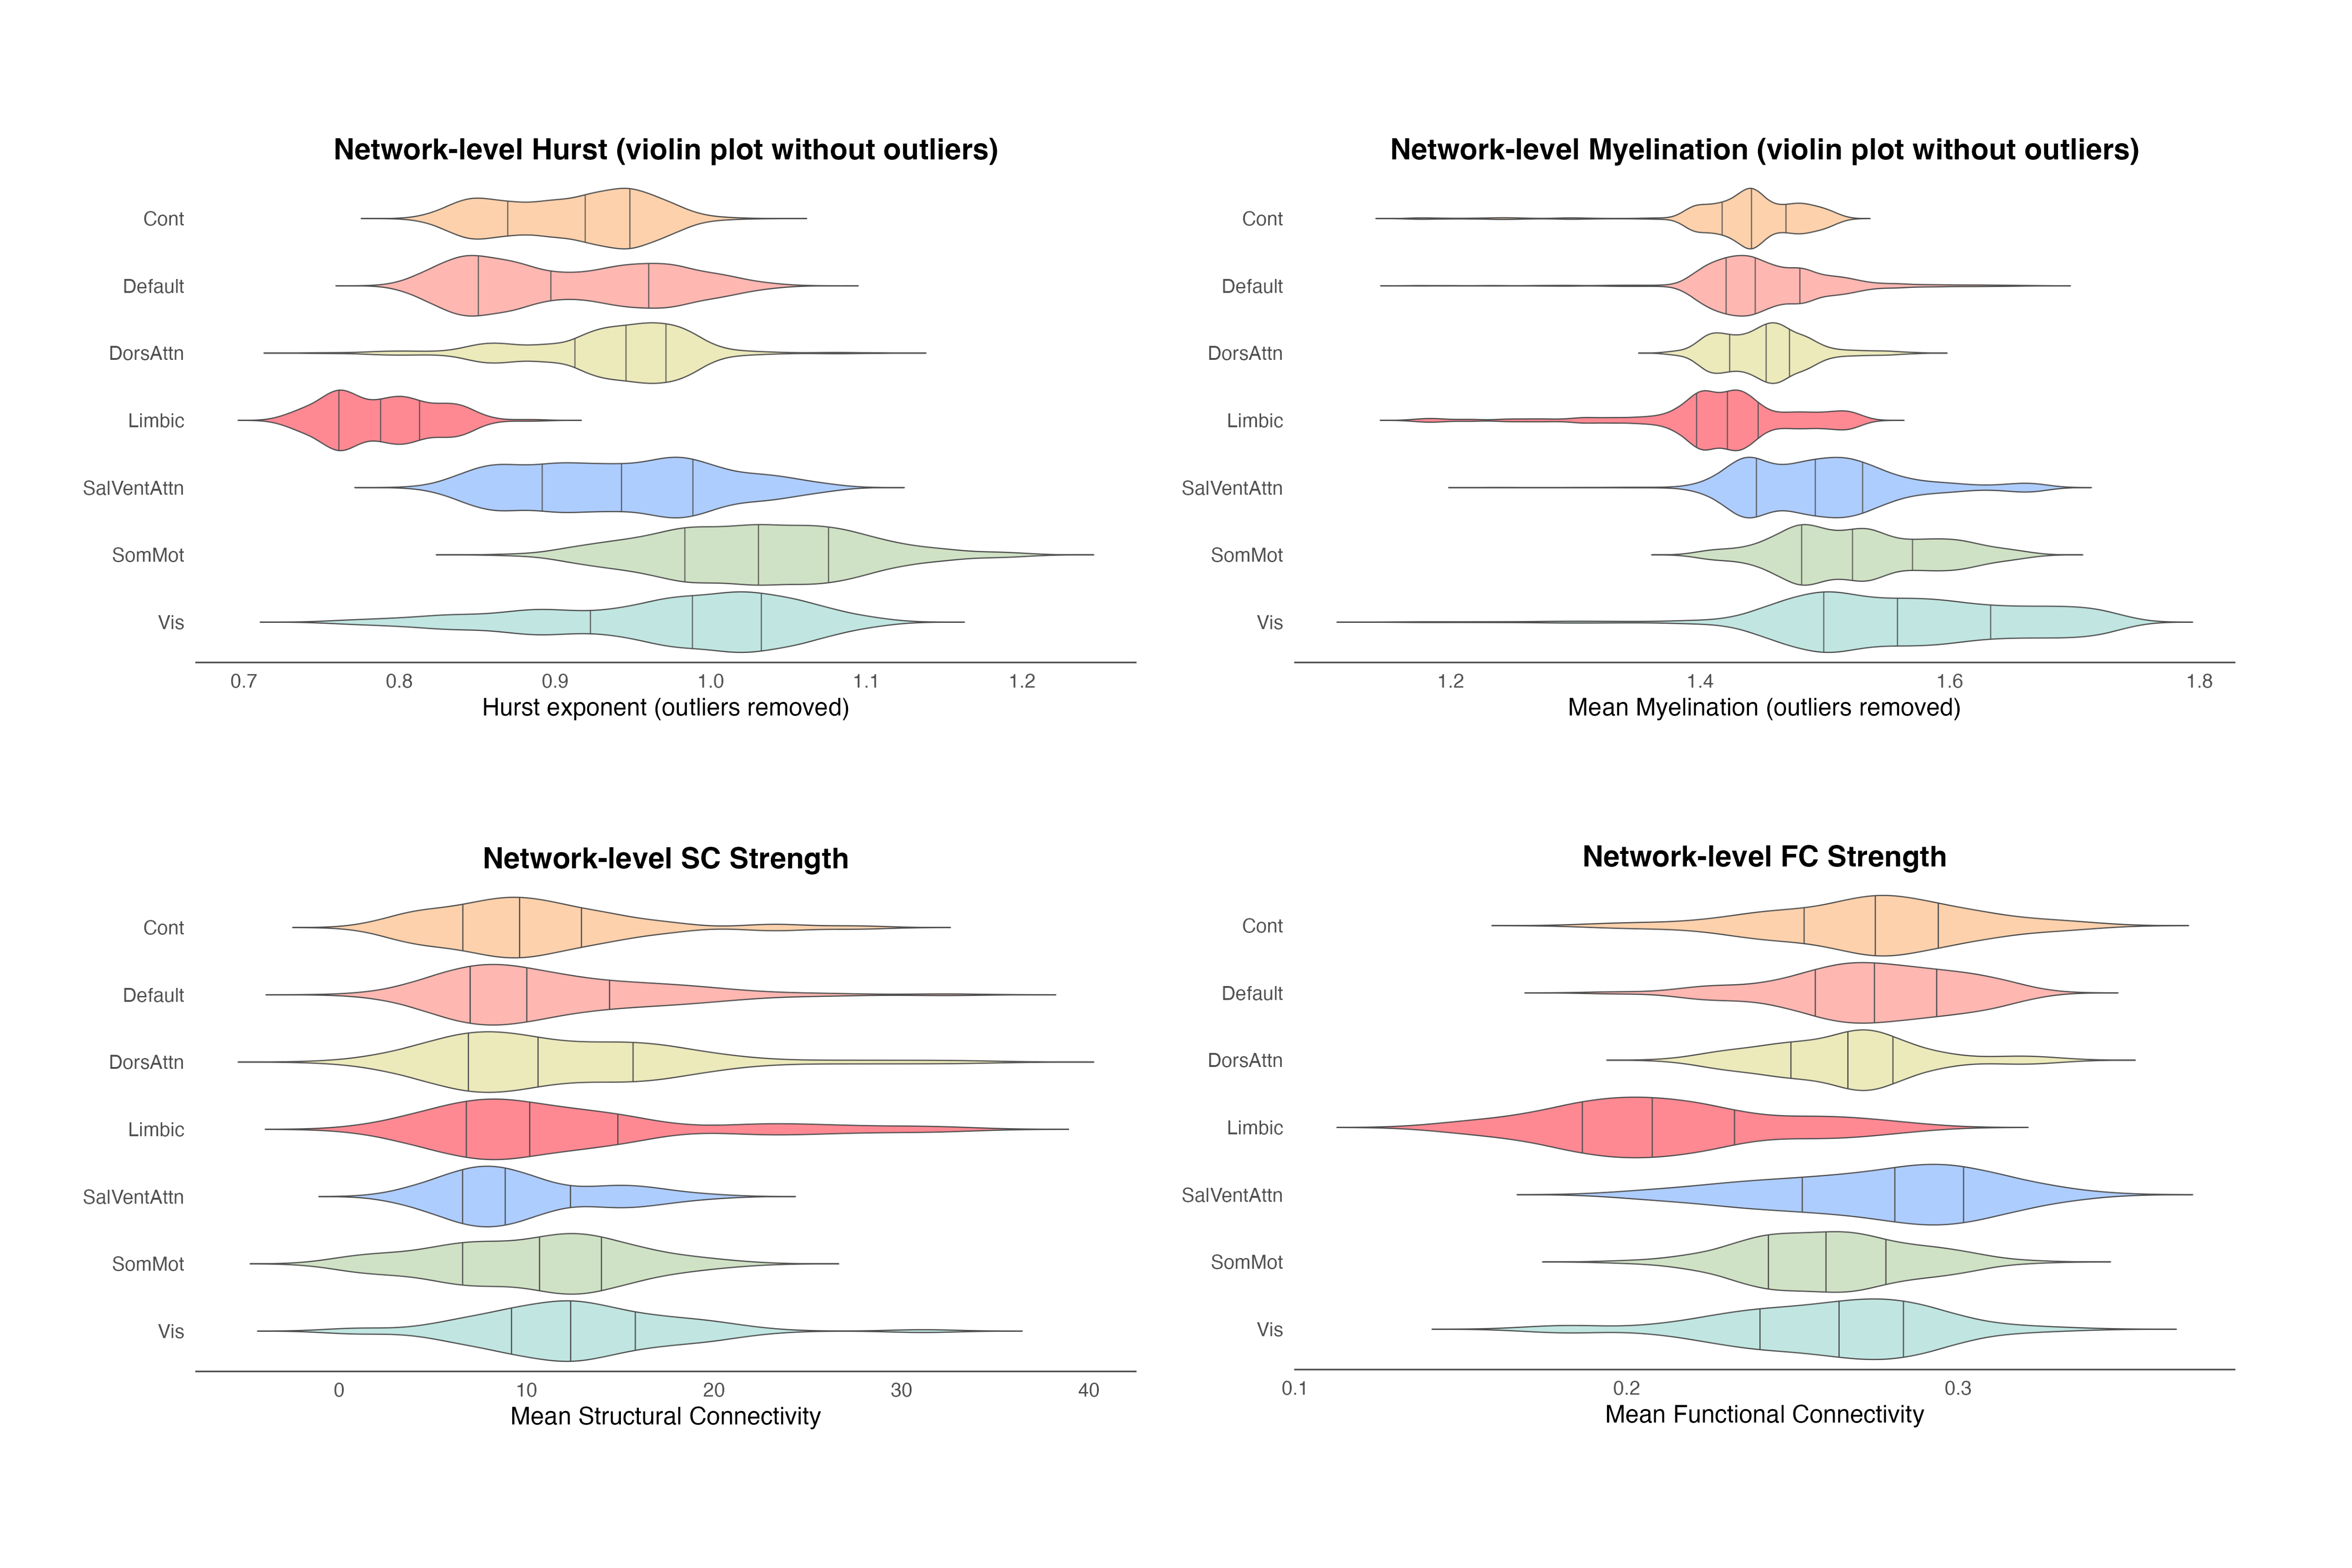
\includegraphics[width=0.95\linewidth]{figure/Figure13_supplementary_net_violin.pdf}
  \caption{\textbf{$|$ Supplementary network-level distributions of SC, FC, and SFC.}
  Violin distributions across canonical networks show stronger intra-network coupling in unimodal systems and weaker coupling in transmodal systems.}
  \label{fig:supplementary_net_violin}
\end{figure}

We defined SC, FC and SFC at the vertex level by constructing individual $20{,}484 \times 20{,}484$ SC and FC matrices from diffusion tractography and vertex-wise BOLD time series for each individual. Next, we derived vertex-wise SFC before mapping all three measures onto the cortical surface (Fig.~\ref{fig:SFC_atlas}a). We then examined the results at three spatial scales---vertices, 400-level ROI, and canonical 7-network partitions---and found that SC, FC and SFC displayed a strikingly homogeneous organization across scales. Group-averaged SC and FC matrices, sorted by canonical networks, exhibited a strongly modular architecture with dense within-network and weaker between-network connectivity, most prominently in unimodal visual (VIS) and somatomotor (SMN) systems (Fig.~\ref{fig:SFC_atlas}b). Chord diagrams of intra-network connections emphasized this pattern, revealing robust reciprocal coupling among unimodal and attentional networks and comparatively sparse connectivity involving limbic cortex (Fig.~\ref{fig:SFC_atlas}c). Longitudinal plots further showed that the strength of these positive intra-network connections increased over infancy and early childhood, with the steepest gains occurring around the first year of life and plateauing thereafter (Extended Data Fig.~\ref{fig:supplementary_FC_Developmental_Trajectory}).

\begin{figure}[t]
  \centering
  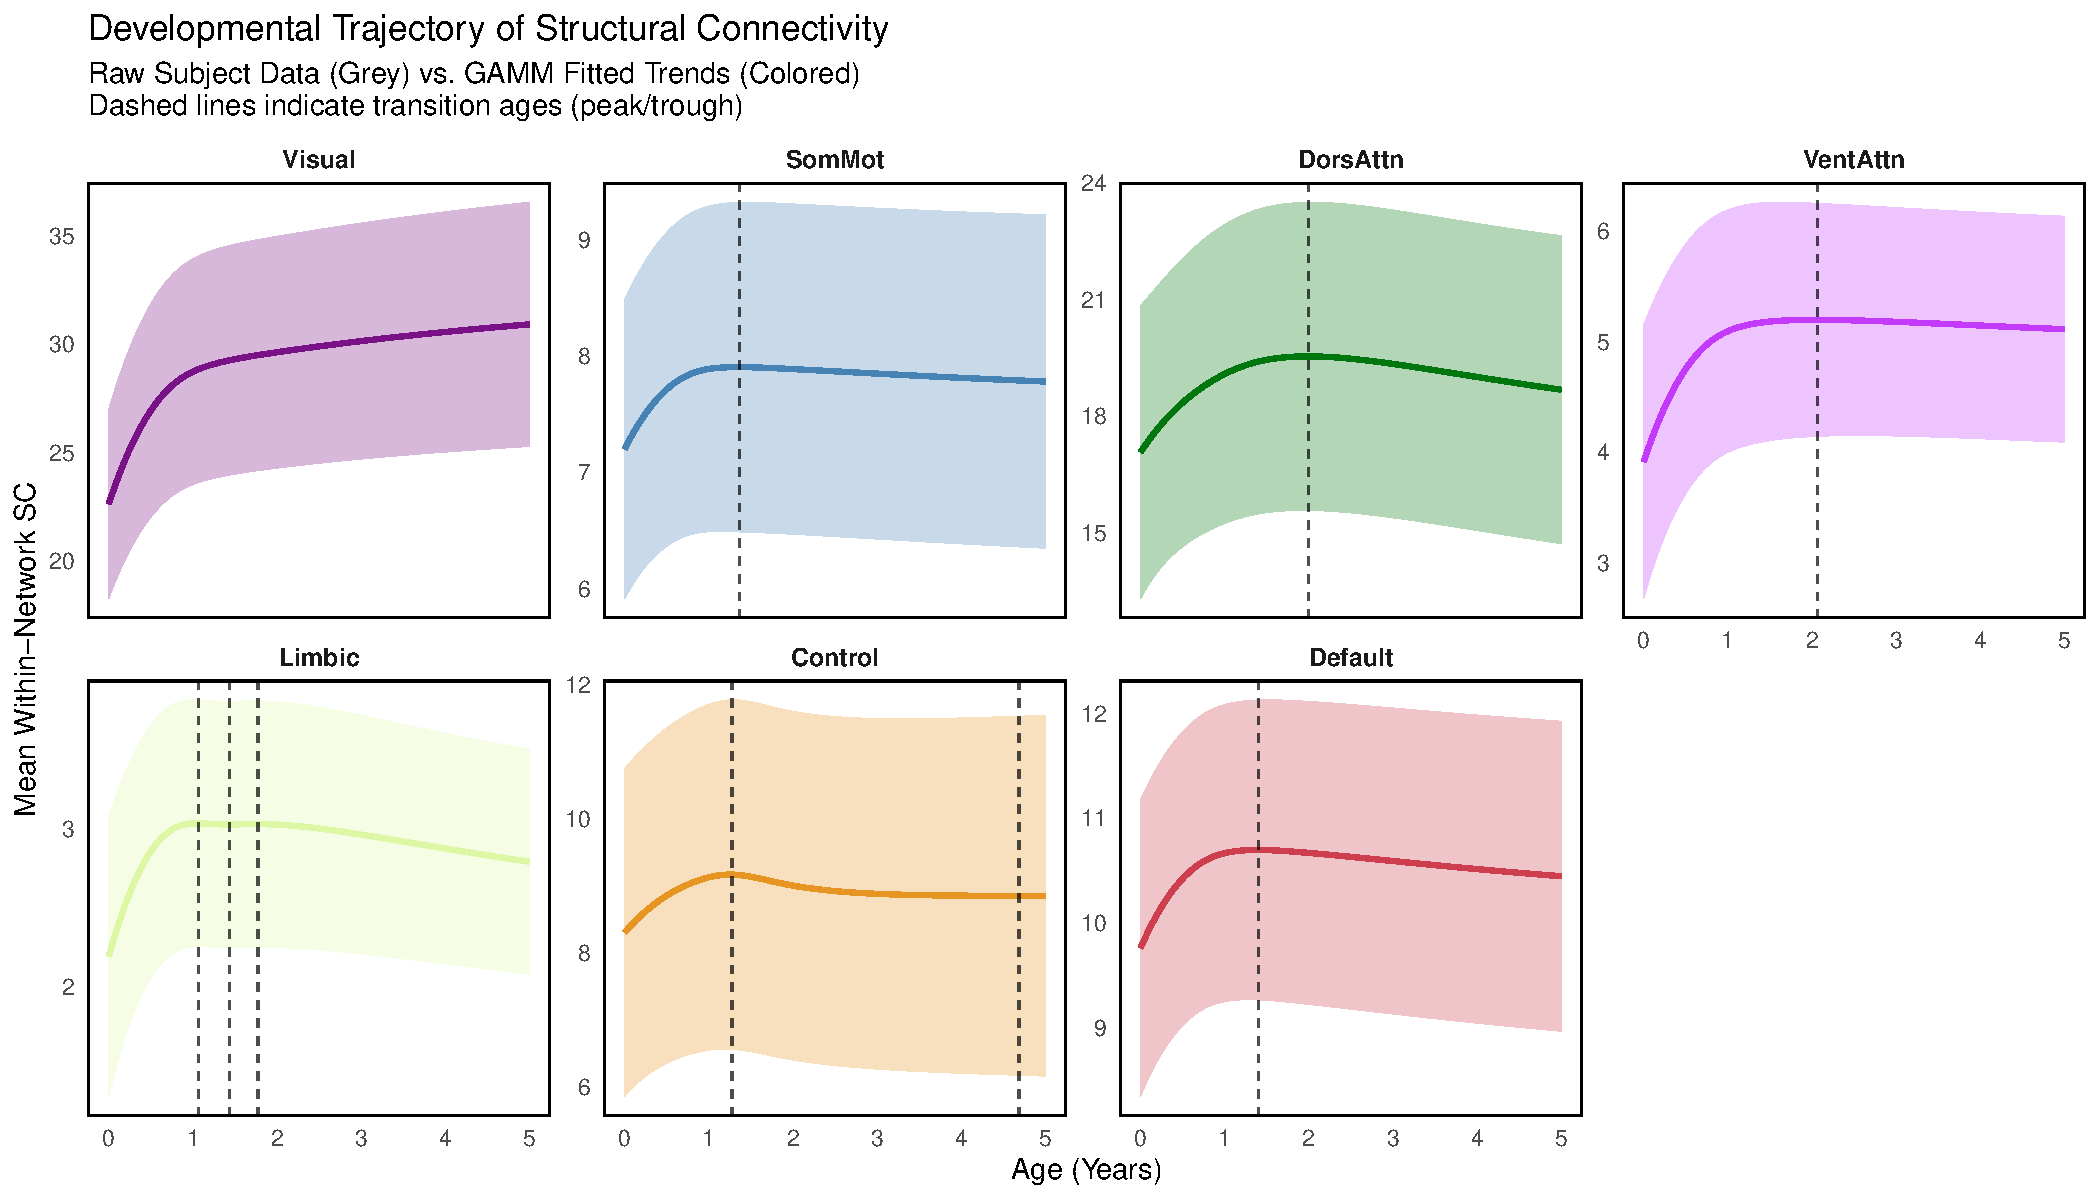
\includegraphics[width=0.95\linewidth]{figure/Figure14_SC_Developmental_Trajectory.pdf}
  \caption{\textbf{$|$ Developmental trajectory of structural connectivity (SC).}
  Longitudinal SC trends across early childhood highlight age-dependent strengthening of structural connections.}
  \label{fig:sc_developmental_trajectory}
\end{figure}

\begin{figure}[t]
  \centering
  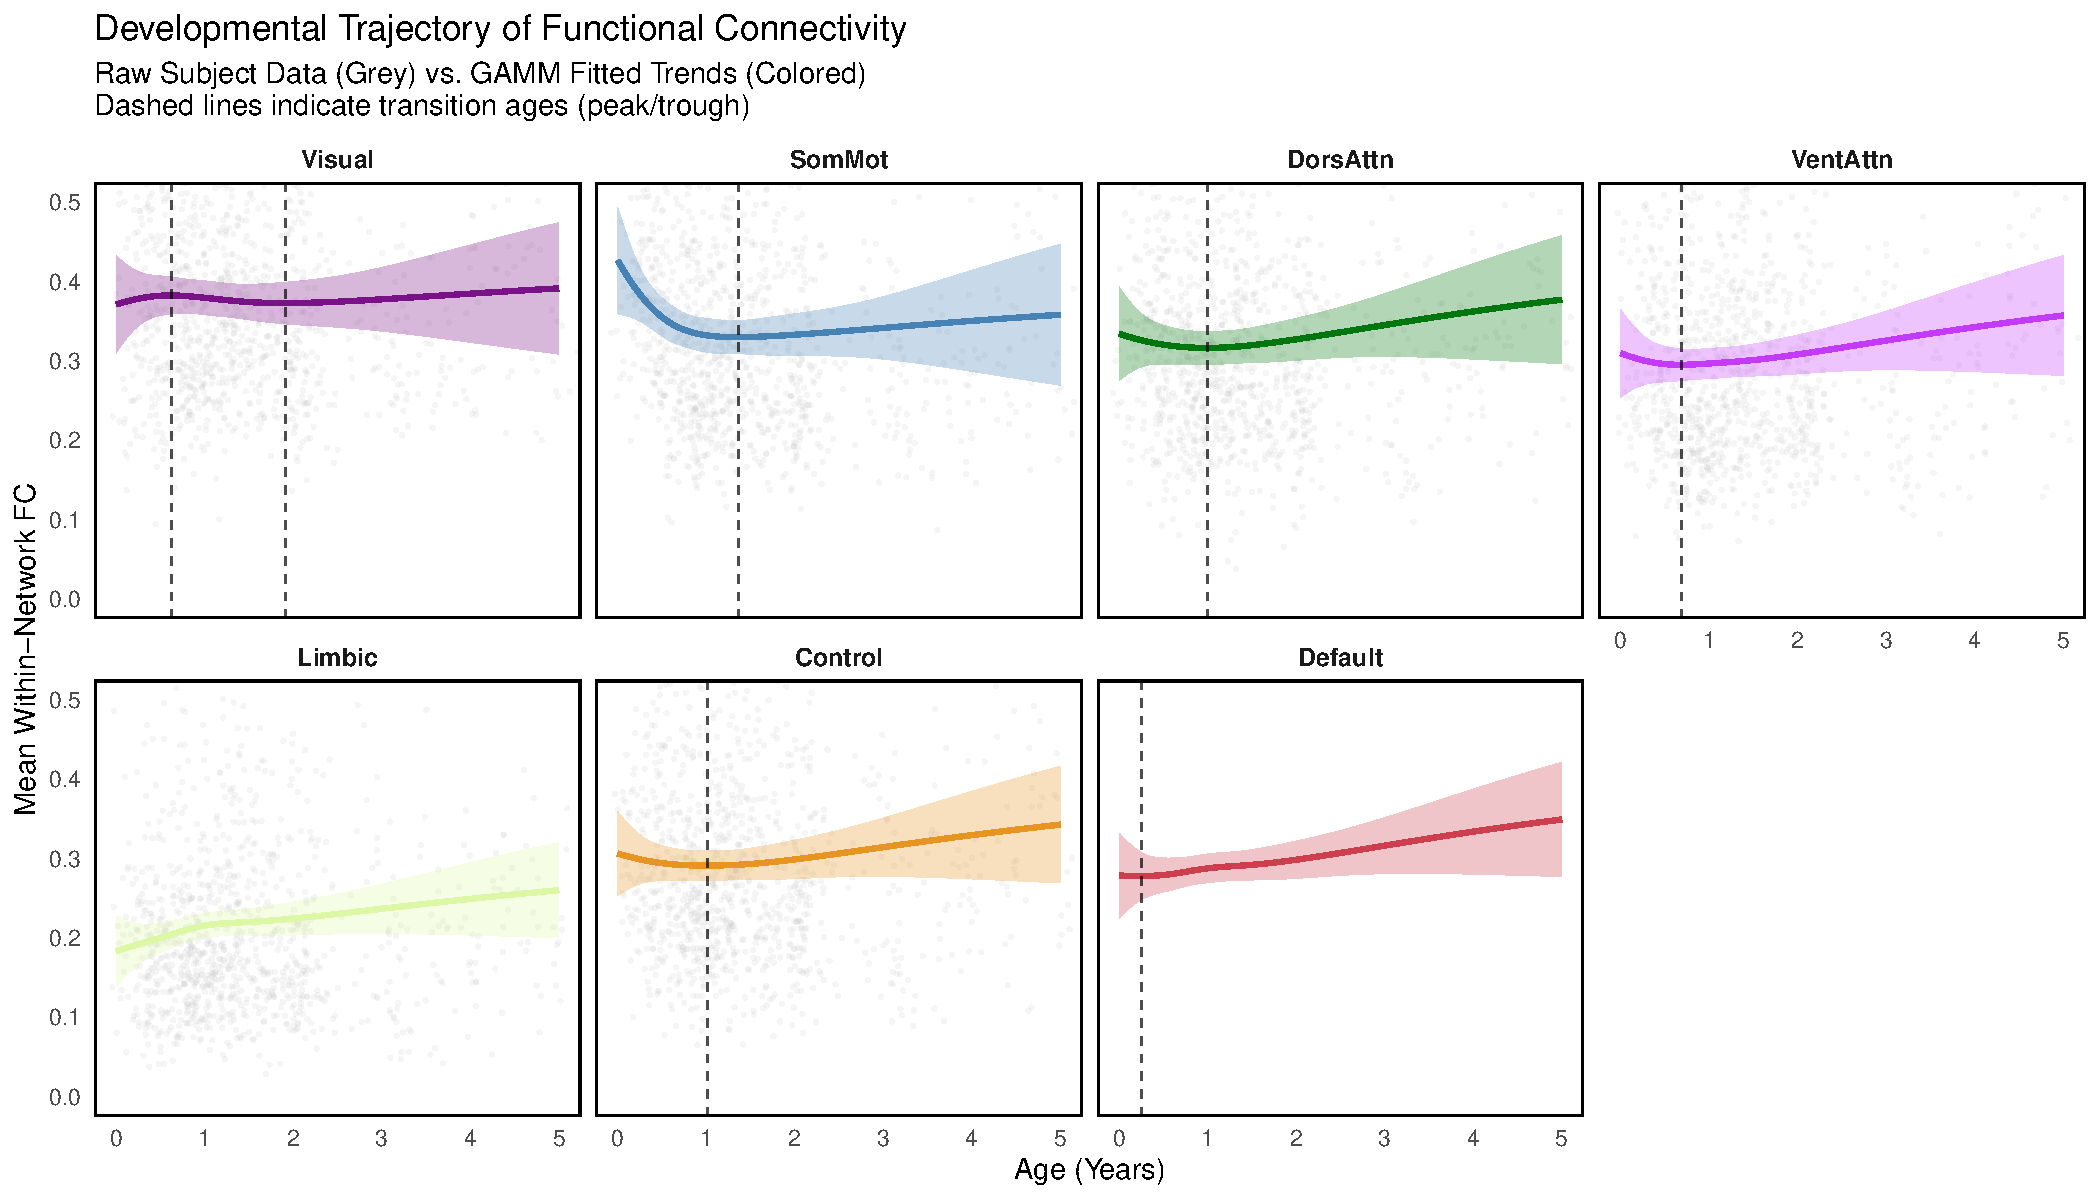
\includegraphics[width=0.95\linewidth]{figure/Figure15_FC_Developmental_trajectory_intra.pdf}
  \caption{\textbf{$|$ Intra-network developmental trajectory of functional connectivity (FC).}
  Longitudinal intra-network FC trends show maturation-related changes in functional coupling across systems.}
  \label{fig:fc_developmental_trajectory_intra}
  \label{fig:supplementary_FC_Developmental_Trajectory}
\end{figure}

Within this modular scaffold, SFC followed a rigid hierarchy. Coupling was strongest in unimodal VIS and SMN networks, intermediate in dorsal and ventral attention (DAN/VAN) and frontoparietal (FP) networks, and weakest in limbic (LIM) and default mode (DMN) systems (Fig.~\ref{fig:SFC_atlas}a). Violin plots of vertex-wise distributions showed that networks with high SFC also had the strongest intra-network SC and FC, whereas transmodal networks with weaker internal SC/FC---especially LIM and DMN---displayed reduced SFC (Extended Data Fig.~\ref{fig:supplementary_net_violin}). Thus, regions that are heavily wired and functionally cohesive exhibit the tightest structure-function alignment, whereas transmodal systems remain more loosely constrained.

Developmentally, this hierarchy was preserved but its magnitude evolved systematically along the S--A axis. Vertex-wise age models revealed widespread increases in SFC from birth to five years, with relatively modest changes in primary sensory and motor regions and marked gains in association cortex (Fig.~\ref{fig:SFC_atlas}e, top). Temporal SFC variance decreased in unimodal cortex but showed more heterogeneous patterns in higher-order networks, consistent with early stabilization of coupling in sensory systems and prolonged reconfiguration in association regions (Fig.~\ref{fig:SFC_atlas}e, bottom). Projecting vertex-wise SC, FC and SFC trajectories onto the continuous S--A gradient clarified these effects (Fig.~\ref{fig:SFC_sa}). Zero-centred SFC trajectories diverged along the axis: sensorimotor vertices began with relatively high coupling that stabilized or slightly declined, whereas association vertices started lower and increased robustly over time (Fig.~\ref{fig:SFC_sa}a). Examining SC and FC within the same S--A bins showed that, at the association (A) end, both SC and FC strengths increased in concert, yielding steadily rising SFC and large positive first derivatives (Fig.~\ref{fig:SFC_sa}b--f). At the sensorimotor (S) end, SC increased rapidly but FC became more selective and, in some cases, decreased relative to the global mean, producing an early mismatch in SC and FC change and modest or negative SFC derivatives. Downsampling the full $20{,}484 \times 20{,}484$ SC and FC matrices into $20 \times 20$ S--A-ordered blocks confirmed that connections involving association vertices carried the largest positive age derivatives in both modalities (Fig.~\ref{fig:SFC_sa}e). Second-derivative analyses further indicated concave-down trajectories (early rise then deceleration) in sensorimotor cortex and more prolonged concave-up trajectories (sustained acceleration) in association cortex (Fig.~\ref{fig:SFC_sa}g--i). Together, these results show that the S--A hierarchy provides a shared coordinate system for the co-development of SC, FC and SFC. Early-maturing sensorimotor cortex is strongly wired and tightly coupled from the outset, whereas later-maturing association cortex undergoes joint structural and functional strengthening that drives progressive increases in structure--function coupling throughout early childhood.

\begin{figure}[t]
  \centering
  \includegraphics[width=0.95\linewidth]{figure/Figure16_SFC_sa.pdf}
  \caption{\textbf{$|$ SFC trajectories along the sensorimotor--association axis.}
  SA-ordered analyses show hierarchical differences in SFC baseline, slope, and curvature from birth to early childhood.}
  \label{fig:SFC_sa}
\end{figure}

\subsection{Excitation--inhibition balance shapes the SFC landscape via temporal dynamics}

\subsubsection{Gradient--E/I coupling (HBCD results)}
The Hurst exponent decreased significantly across the cortex from 1 week to 6 months, with the largest decreases in sensorimotor and visual regions, spatially overlapping with areas of strongest gradient maturation. Network-level analyses confirmed that somatomotor and visual networks exhibited the highest within-network variance, reflecting heterogeneous E/I development (Fig.~\ref{fig:hurstgradient_hbcd}a). GAMM-fitted trajectories revealed a sharp initial decline in Hurst exponent across all networks, with the steepest decrease occurring in the first 6 weeks. The first derivative showed peak acceleration around 6 weeks, followed by stabilization at approximately 3 months (Fig.~\ref{fig:hurstgradient_hbcd}c). Functional gradient maturation was spatially coupled with shifts in local E/I balance. Vertex-wise analyses revealed negative correlations between Hurst exponent and both S--A (\(r = -0.335\)) and V--S (\(r = -0.289\)) gradients: regions at the primary ends of both gradients exhibited lower Hurst values, indicating higher E/I ratio. This coupling strengthened over development, with correlation slopes becoming steeper by 6 months (Fig.~\ref{fig:hurstgradient_hbcd}b). Regions showing the strongest gradient differentiation also exhibited the largest Hurst decreases.

These findings demonstrate that functional gradient differentiation and excitation-inhibition dynamics are spatially coupled during early infancy, with primary sensory regions showing both the strongest gradient maturation and the largest shifts toward excitation dominance. This coupling suggests that local physiological changes in E/I balance may drive the emergence of macroscale functional organization. The developmental trajectory follows a sensorimotor-first pattern: primary regions differentiate rapidly in the first 6 weeks before stabilizing, while association cortices lag behind, consistent with hierarchical models of cortical maturation. Our vertex-level framework, combining functional gradient analysis with Hurst exponent mapping, enables fine-scale characterization of neurophysiology in the infant brain. Applied to the HBCD cohort, this approach establishes normative trajectories of gradient--E/I coupling that may facilitate early detection of atypical patterns implicated in neurodevelopmental disorders. As longitudinal HBCD data become available, this framework will enable tracking of individual developmental trajectories across infancy.

\begin{figure}[t]
  \centering
  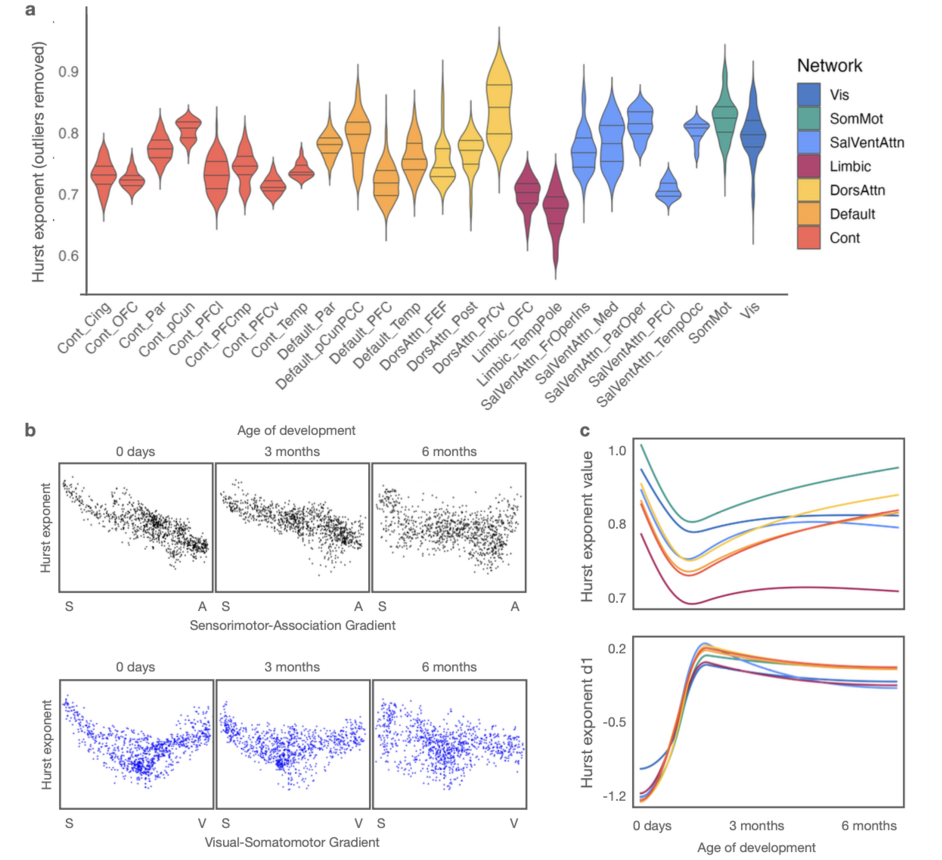
\includegraphics[width=0.95\linewidth]{figure/Figure17_Hurstgradient_HBCD.png}
  \caption{\textbf{$|$ Network-level organization and dynamics of E/I balance across early postnatal development.}
  (a) Hurst exponent distributions across Schaefer 400 parcels. Primary networks (visual, somatomotor) show higher average Hurst values, suggesting relatively lower excitation--inhibition (E/I) balance. (b) Scatter plots showing the relationship between functional gradients (SA, VS) and Hurst exponent across development. At each age point, 1,000 vertices were randomly sampled from the cortical surface (10k mesh). A negative association emerges and strengthens with age, particularly at the sensorimotor and visual ends of each gradient. (c) Top: Network-averaged Hurst exponent trajectories over the first 6 months of life. Bottom: First derivative of Hurst exponent over age, showing peak rate of change at $\sim$6 weeks across all networks, with strongest early decline in primary systems.}
  \label{fig:hurstgradient_hbcd}
\end{figure}

\begin{figure}[t]
  \centering
  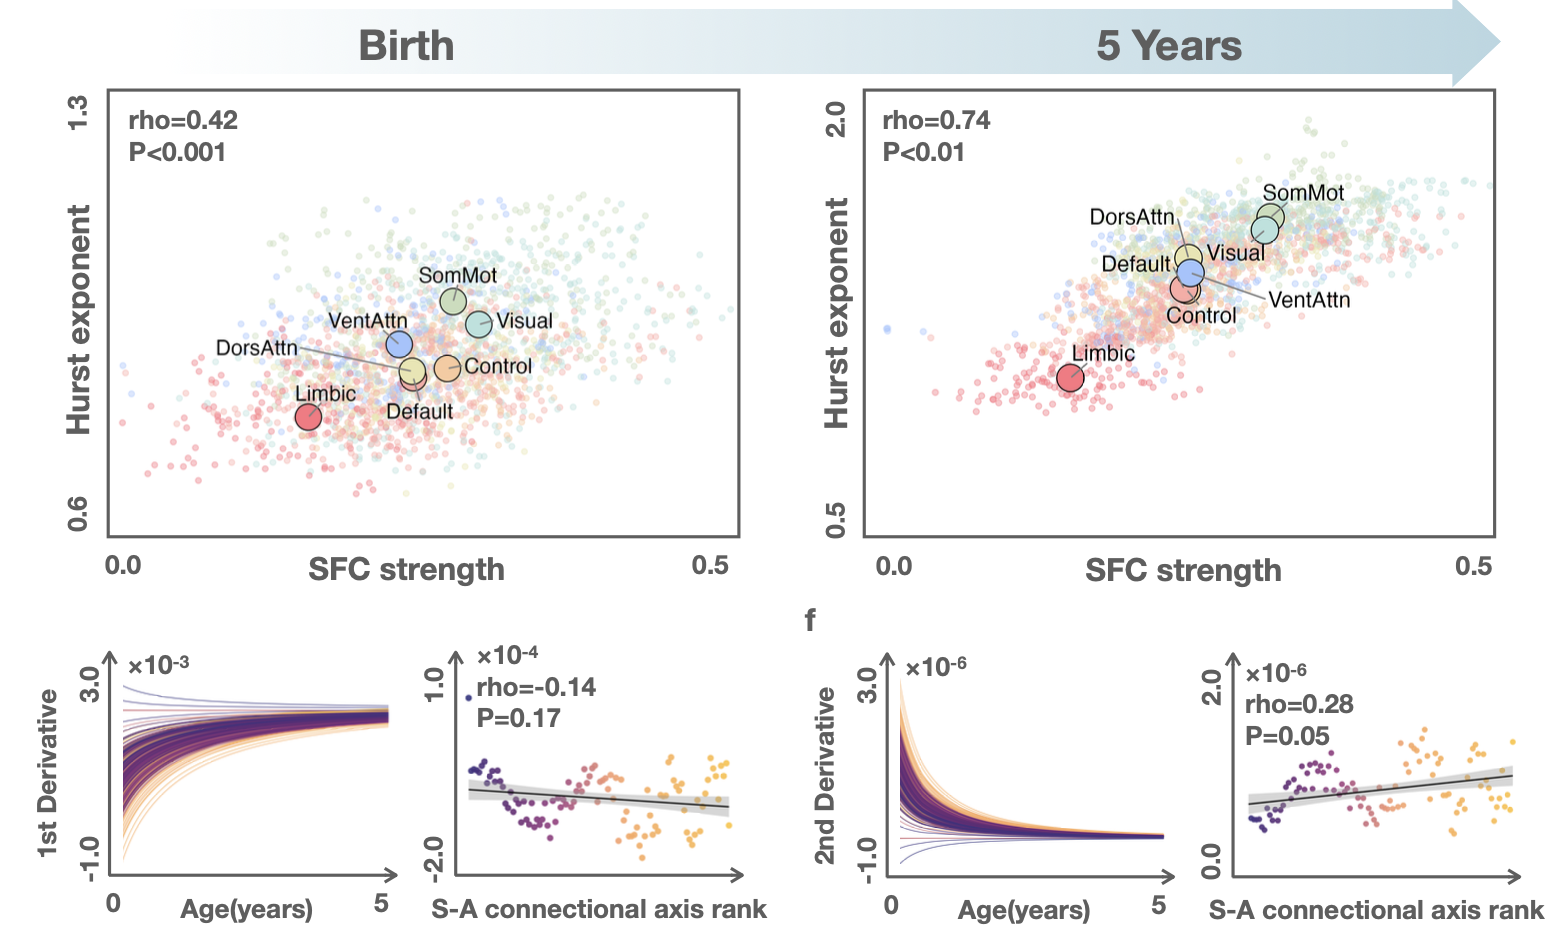
\includegraphics[width=0.95\linewidth]{figure/Figure18_Hurstsa_BCP.png}
  \caption{\textbf{$|$ Hurst trajectory along the S--A axis in BCP.}
  Developmental patterns of Hurst exponent along the sensorimotor--association hierarchy in the BCP cohort.}
  \label{fig:hurstsa_bcp}
  \label{fig:Hurst_sa}
  \label{fig:hurst_sa}
\end{figure}

We next asked how local temporal dynamics contribute to the emergence of structure-function coupling. For each subject and vertex, we estimated the Hurst exponent ($H$) of the resting-state BOLD signal on the cortical surface, using it as a proxy for excitation-inhibition (E/I) balance, where lower $H$ reflects faster, more stochastic dynamics (higher E/I ratio) and higher $H$ reflects slower, more autocorrelated dynamics (lower E/I ratio). Across 0 to 5 years, mean $H$ declined globally, indicating a developmental shift toward higher E/I ratios, with earlier stabilization in sensorimotor cortex and more prolonged, nonlinear change in transmodal association regions (Fig.~\ref{fig:Hurst_sa}a–d). To relate these trajectories to the sensorimotor-association (S-A) hierarchy, we projected an established S–A gradient onto the infant cortical surface by matching each vertex to an adult template and then grouping vertices into 100 equally sized bins along the gradient (purple = lowest S-end, yellow = highest A-end). For each bin, we computed the mean first and second derivatives of the fitted $H$ curves across 0 to 5 years; plotting these 100 bin averages yielded the SA-ordered line and scatter plots in Fig.~\ref{fig:Hurst_sa}e,f. Curvature of $H$ trajectories varied systematically along the axis (second derivative vs.\ S-A rank, Spearman's $\rho \approx 0.28$, $p \approx 0.05$; Fig.~\ref{fig:Hurst_sa}f), consistent with extended remodeling of temporal dynamics in association cortex.

We then examined how the spatial coupling between $H$ and SFC strengthens over development. At birth, the vertex-wise scatter of SFC versus $H$ was broad and diffuse, with only a modest positive relationship and considerable overlap across networks. By age five, points clustered tightly along a steeper positive trend, and the network centroids followed a clear hierarchy: primary visual and somatomotor systems showed the highest SFC and $H$, followed by attention and control networks, with limbic and default mode regions occupying the low-SFC, low-$H$ end of the continuum. Correspondingly, the spatial correlation between mean SFC and mean $H$ increased from infancy to preschool ($\rho_{\text{birth}} \approx [0.42]$ to $\rho_{\text{5y}} \approx [0.74]$), indicating that regions that maintain slower, more autocorrelated dynamics increasingly become the ones whose functional coupling most closely tracks structural wiring. This association remained robust after accounting for position along the S-A axis and intracortical myelination (partial Spearman’s $\rho \approx 0.56$, $p < 10^{-4}$), suggesting that E/I-related temporal regimes provide a functional component that independently shapes how tightly structure and function are coupled during early childhood.


\subsection{Intracortical myelination tracks the emergence of SFC}
We also found that structural maturation (intracortical myelination), indexed by the T1w/T2w ratio, helps explain this hierarchical pattern of SFC during the first 5 years of life. Myelination in sensorimotor cortex exhibited rapid, early-saturating increases, whereas association cortex showed slower but more sustained growth across the 0–5 year window (Fig.~\ref{fig:myelin_sa}c–f). First-derivative analyses confirmed steeper early myelin gains in low-rank (sensorimotor) regions and more prolonged increases in high-rank (association) regions (Spearman’s $\rho \approx 0.57$, $p < 0.001$; Fig.~\ref{fig:myelin_sa}e), consistent with classic myelogenetic sequences.

\begin{figure}[t]
  \centering
  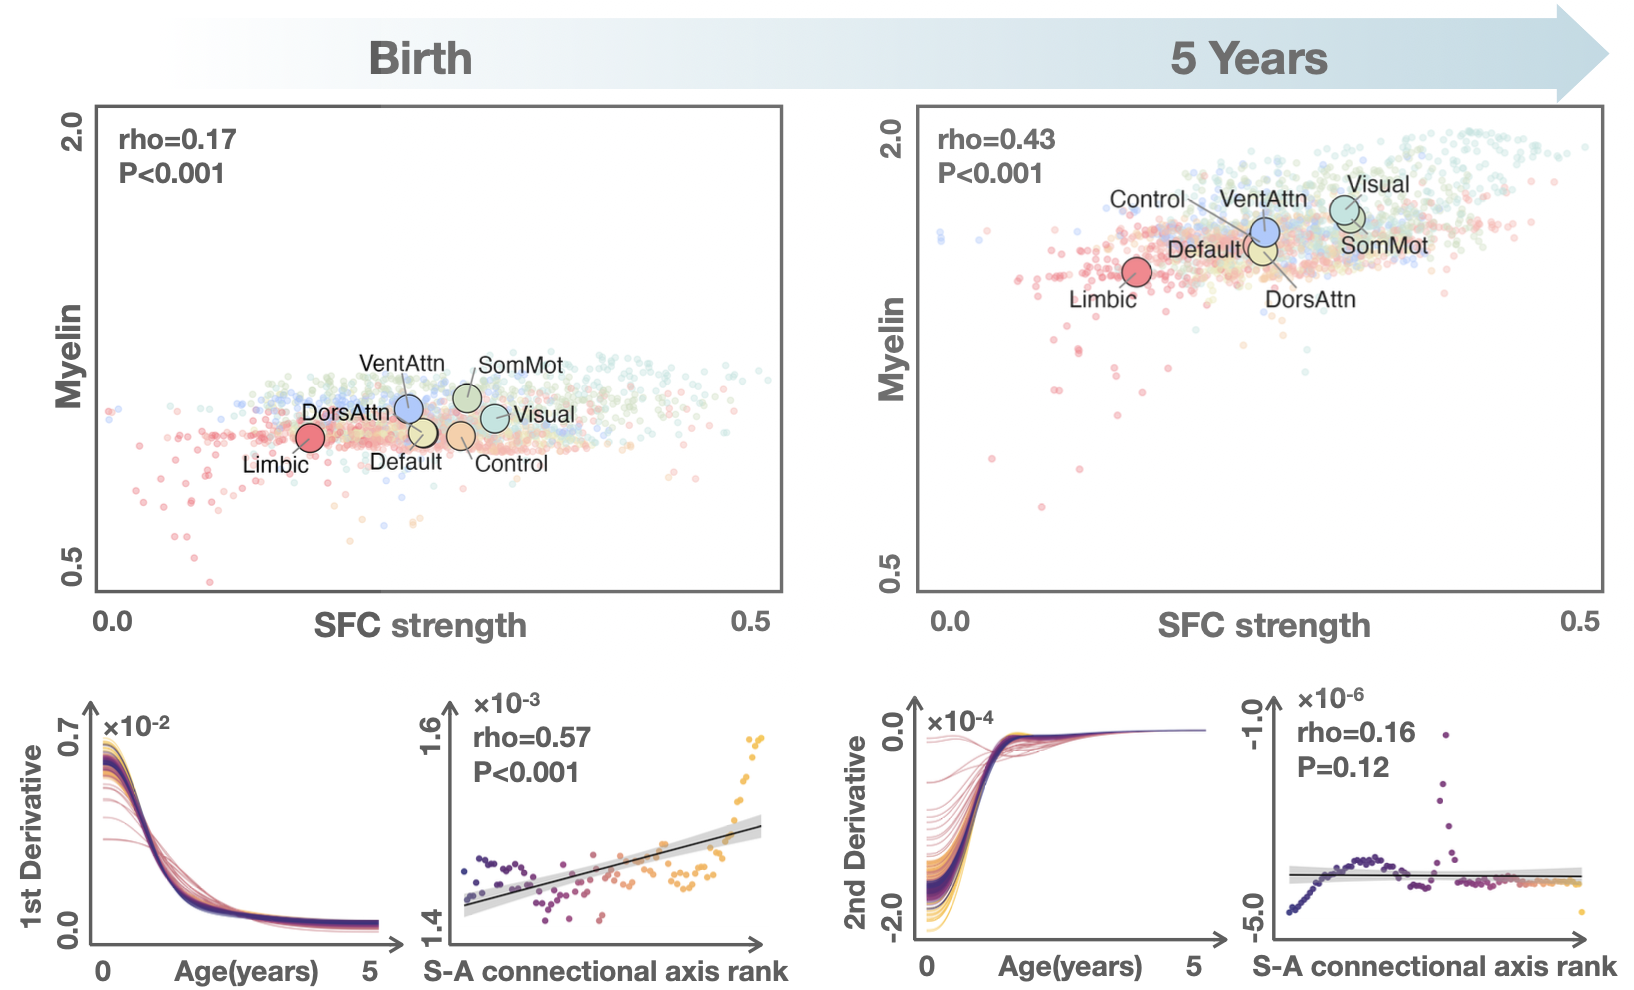
\includegraphics[width=0.95\linewidth]{figure/Figure19_myelinsa_BCP.png}
  \caption{\textbf{$|$ Myelination trajectory along the S--A axis in BCP.}
  Developmental pattern of intracortical myelination along the sensorimotor--association hierarchy in early childhood.}
  \label{fig:myelinsa_bcp}
  \label{fig:myelin_sa}
\end{figure}

Spatial coupling between myelination and SFC strengthened over development, but with a different profile than for $H$. At birth, SFC–myelin scatterplots showed only weak alignment, with considerable dispersion and limited separation across networks. By age five, points became more tightly distributed around a positive regression line, and network means fell into a familiar hierarchy: unimodal visual and somatomotor systems again occupied the high-myelin, high-SFC end, attentional and control networks were intermediate, and limbic/default regions remained low on both axes. The corresponding vertex-wise correlation between SFC and myelin increased from early infancy to preschool ($\rho_{\text{birth}} \approx [0.17]$ to $\rho_{\text{5y}} \approx [0.43]$), indicating that as the cortical scaffold matures, regions with denser intracortical myelin are increasingly those in which functional interactions most closely follow structural connectivity.

In conclusion, this SFC-myelin relationship partly reflects shared organization along the S-A axis and with E/I-related dynamics, but myelin also explains unique variance. After controlling for S-A rank and $H$, the spatial association between SFC and myelin remained significant, albeit attenuated (partial Spearman's $\rho \approx 0.18$, $p < 10^{-4}$). Together with the Hurst findings, these results support a dual-component view in which intracortical myelination supplies a slowly evolving structural scaffold, while E/I-related temporal regimes provide a functional constraint; the intersection of these two components determines where, and how strongly, cortical structure and function become locked together during early childhood.



\subsection{Microstructure and excitation--inhibition balance gate how SC and FC co-development expresses as SFC}

Finally, we asked how the co-development of structural and functional connectivity along the S--A axis is shaped by local microstructure and neural dynamics. Because SFC is defined as the correlation between each vertex's SC and FC profiles, its maturation should depend not only on how strongly SC and FC grow, but also on whether this growth occurs in a microcircuit context that favors stable, structurally constrained dynamics. We therefore related vertex-wise SFC to intracortical myelination (T1w/T2w) and the Hurst exponent, both in space and in time, leveraging the same vertex-level maps used in the SA and network analyses (Figs.~\ref{fig:timeline}, \ref{fig:myelin_sa}, \ref{fig:hurst_sa}).

Across the cortical sheet, SFC was strongly coupled to intracortical myelination: vertices with higher T1w/T2w ratios exhibited systematically stronger SFC (Spearman's $r = 0.658$, $p < 0.001$). A similarly strong spatial relationship was observed between SFC and the Hurst exponent: regions with higher H (more temporally autocorrelated, inhibitory-like dynamics) showed higher SFC (Spearman's $r = 0.640$, $p < 0.001$), suggesting that slower, more stable intrinsic dynamics support tighter locking of FC to the underlying SC scaffold.

We then examined whether vertices whose SFC trajectories changed most over time were the same vertices in which myelination and E/I-related dynamics changed in synchrony. For each vertex, we computed the temporal correlation between its GAMM-fitted SFC trajectory and its myelin trajectory from birth to 5 years (Methods). Positive temporal correlations clustered in higher-order association and dorsal attention cortex (for example, vertex V3498: $r = 0.207$), where gradual increases in T1w/T2w paralleled progressive strengthening of SFC. In contrast, some sensorimotor vertices showed weak or negative temporal coupling (for example, V2100: $r = -0.185$), consistent with our SA analyses: in these early-maturing regions, rapid early myelination is followed by FC refinement that temporarily reduces SC--FC alignment before stabilizing (Figs.~\ref{fig:SFC_sa}, \ref{fig:myelin_sa}). Thus, even where SFC and myelin are positively related in space, their temporal co-evolution can diverge across the hierarchy.

An analogous pattern emerged for SFC and the Hurst exponent. Vertex-wise temporal correlations between SFC and H were generally positive but heterogeneous: association and control regions often showed modest positive coupling (for example, V1506: $r = 0.209$), such that vertices that maintained higher H (or slowed their decline in H) also exhibited larger gains in SFC. In contrast, some visual vertices showed near-zero temporal coupling (for example, V3498: $r = 0.014$), implying that once SFC is established in unimodal cortex, ongoing changes in E/I-related dynamics have limited additional impact on structure--function alignment. Importantly, the positive spatial association between SFC and H remained significant after adjusting for myelin and S--A rank, indicating that microstructure and dynamics make partially independent contributions to the SFC landscape.

Taken together, these multimodal analyses show that the same S--A hierarchy that organizes the co-development of SC, FC and SFC also shapes how local microstructure and E/I-related dynamics gate this co-development. In early-maturing sensorimotor cortex, rapid myelination and evolving, increasingly desynchronized dynamics support strong but relatively inflexible SFC that can transiently weaken as FC refines. In later-maturing association cortex, prolonged myelination and the maintenance of more autocorrelated dynamics provide a permissive regime in which co-increases in SC and FC translate into steadily rising SFC. Thus, along the cortical hierarchy, SFC emerges from the coordinated maturation of anatomical wiring, functional coupling, and local circuit properties, providing an integrated marker of how structural and functional hierarchies co-develop in early childhood.


\section{Discussion}
% finding
In this study, we leveraged vertex-wise multimodal MRI from birth to five years of age to chart how structural and functional hierarchies co-develop to shape structure–function coupling in the human cortex. Across this critical window, we observed a pronounced global strengthening of structure–function coupling (SFC) accompanied by parallel increases in intracortical myelination and a shift toward faster, more desynchronized temporal dynamics indexed by the Hurst exponent. Importantly, these changes were not spatially uniform: SFC, structural connectivity (SC), functional connectivity (FC), myelination, and Hurst all exhibited systematic variation along the sensorimotor–association (SA) axis, with unimodal systems showing early, high coupling and association systems displaying delayed and protracted refinement. Together, these findings reveal that the SA hierarchy provides a common developmental scaffold along which cortical wiring, microstructure, and dynamics are jointly tuned, establishing the early architecture that will later support specialized cognition and potentially confer vulnerability to atypical trajectories.

We demonstrate that functional gradient differentiation and excitation-inhibition dynamics are spatially coupled during early infancy, with primary sensory regions showing both the strongest gradient maturation and the largest shifts toward excitation dominance. This coupling suggests that local physiological changes in E/I balance may drive the emergence of macroscale functional organization. The developmental trajectory follows a sensorimotor-first pattern: primary regions differentiate rapidly in the first 6 weeks before stabilizing, while association cortices lag behind, consistent with hierarchical models of cortical maturation. Our vertex-level framework, combining functional gradient analysis with Hurst exponent mapping, enables fine-scale characterization of neurophysiology in the infant brain. Applied to the HBCD cohort, this approach establishes normative trajectories of gradient-E/I coupling that may facilitate early detection of atypical patterns implicated in neurodevelopmental disorders. As longitudinal HBCD data become available, this framework will enable tracking of individual developmental trajectories across infancy.

We further demonstrate that OS-SVD enables high-quality individual gradients that align with population-level patterns. Across denoising benchmarks, OS-SVD provided the strongest improvement in temporal SNR while preserving structural information in residual maps, and it remained robust under temporally undersampled acquisitions. These results indicate that individual gradients can be reliably obtained with under 4 minutes of rs-fMRI acquisition time, supporting faster and more practical infant imaging protocols.

% SC-> SFC, FC -> sFC 
A central implication of our findings is that the unimodal-transmodal gradient provides a common scaffold for the co-development of structural and functional hierarchies that jointly shape SFC. This interpretation is supported by studies using definitions of SFC other than the correlational approach here. For instance, (i) harmonic decomposition of the connectome expresses BOLD signals in graph-frequency space, with structure-function decoupling defined by the ratio of high (decoupled) to low (coupled) frequency components\cite{vazquez-rodriguezGradientsStructureFunction2019,liuTimeresolvedStructurefunctionCoupling2022}, and (ii) in predictive regression frameworks, SFC is indexed by how well a region's empirical FC can be explained from structural features such as Euclidean distance, shortest path length, and communicability derived from the connectome. These complementary methods converge on a heterogeneous pattern of structure-function decoupling along the sensory-association hierarchy, indicating that the phenomenon is robust across analytic definitions of SFC. Notably, it is also robust across developmental stages: prior work in adults and older youth has shown the gradual decoupling of function from structure along the unimodal-transmodal gradient\cite{marguliesSituatingDefaultmodeNetwork2016,fotiadisMyelinationExcitationinhibitionBalance2023,suarezLinkingStructureFunction2020a,guHeritabilityInterindividualVariability2021}, and our vertex-wise analyses extend this principle into the first five years of life, demonstrating that SFC, SC, and FC already obey a shared S-A hierarchy during a period of rapid cortical maturation.

The unimodal-transmodal axis has been proposed as a principal coordinate system that captures the developmental chronology of multiple neurobiological properties, including structural connectivity strength, functional connectivity organization, intracortical myelination, and intrinsic activity timescales\cite{sydnorNeurodevelopmentAssociationCortices2021,xuStructuralConnectivityMatures2024,fotiadisMyelinationExcitationinhibitionBalance2023}. Echoing longitudinal tractography work in older children and adolescents, we observed that unimodal visual and somatomotor systems are both strongly wired and tightly structure-function coupled from early in life, whereas attentional, control, default mode, and limbic networks occupy higher positions along the SA axis, with weaker initial SFC but more protracted strengthening\cite{lebelLongitudinalDevelopmentHuman2011}.  These results suggest that the SA hierarchy not only organizes the mature connectome, but also governs the temporal ordering with which structural constraints and functional specialization are imposed during early stages of development.

% thus, proof of myeliation correlation , myeliation ->SC -> SFC
A second implication of our findings is that hierarchical differences in SFC appear to arise from the coordinated maturation of structural and functional components of cortical circuitry. In our framework, intracortical myelination serves as a proxy for the structural substrate that supports communication, whereas the Hurst exponent indexes local functional dynamics related to excitation-inhibition (E/I) balance.

%H relate with I in one paper, they find H + from 4-5 but they do 400 ROI 
The functional component indicates that heterogeneity in excitation/inhibition balance is inversely related to structure--function coupling. Regions with higher Hurst exponents---reflecting more temporally autocorrelated dynamics and lower E/I ratios---tended to exhibit stronger and less temporally variable SFC. Because the E/I ratio is defined as excitation relative to inhibition, lower E/I values correspond to relatively stronger inhibitory influence; under this interpretation, our observed positive Hurst--SFC relationship supports a direct link between inhibitory-dominant regimes and tighter SC--FC alignment. Developmentally, Hurst values decreased across 0--5 years, indicating a shift toward higher E/I ratios (greater relative excitation), with the most pronounced changes occurring in the first six months of life (Fig.~\ref{fig:hurst_sa}). Notably, both the absolute range and the direction of Hurst changes that we observe are consistent with recent developmental work reporting rapid decreases in scale-free exponents during infancy and early childhood\cite{stanyardAperiodicHurstEEG2024a,houtmanSTXBP1SyndromeCharacterized2021,nishioHurstExponentMarker2024}. We treat Hurst as an index of E/I-related temporal dynamics, but acknowledge that in early development it likely reflects a composite of changes in excitation, inhibition, conduction speed, and global brain state. Taken together with the myelination findings, our results support a view in which SFC in early childhood is jointly shaped by a structural component (intracortical myelination) and a functional component (E/I-related dynamics), whose coordinated but non-uniform maturation underlies the emergent hierarchy of structure--function alignment.
% Consistent with this view, microcircuit studies and modeling work have shown that both excitatory receptor composition and inhibitory interneuron architecture systematically vary along the cortical hierarchy, and that regional differences in Hurst and related 1/f measures covary with inhibitory markers, including parvalbumin (PV$^{+}$) interneuron gene expression\cite{nishioHurstExponentMarker2024}.
% From unimodal sensory and motor areas to heteromodal association cortex, there is a progressive increase in synaptic excitation, supported by greater dendritic complexity and spine density, as well as higher expression of GluN2B-containing NMDA receptors that mediate slow-gating excitatory transmission and support prolonged integration and persistent firing, particularly in prefrontal neurons\cite{wangMacroscopicGradientsSynaptic2020a,FotiadisBiological2026,hensonDevelopmentalRegulationNMDA2008}.
% In contrast, primary sensory regions rely more heavily on fast AMPA receptor-mediated transmission, which is better suited to rapid encoding of sensory inputs and efficient bottom-up signal propagation\cite{wangMacroscopicGradientsSynaptic2020a,YangSynaptic2018}.
% A parallel shift is observed in inhibitory circuitry: in unimodal cortex, inhibition is dominated by PV$^{+}$ parvalbumin-expressing interneurons that target perisomatic compartments and tightly regulate spike output, whereas in association cortex a larger proportion of inhibition is mediated by CB$^{+}$ calbindin- and CR$^{+}$ calretinin-expressing interneurons that innervate distal dendrites and gate the integration of convergent long-range and neuromodulatory inputs\cite{gonzalez-burgosFunctionalMaturationGABA2015,fishParvalbuminContainingChandelierBasket2013,fungExpressionInterneuronMarkers2010}.
% Together, these gradients in excitatory receptor composition and inhibitory targeting provide a mechanistic substrate for the more persistent, integrative dynamics indexed by higher Hurst exponents in association cortex, and help explain why developmental changes in E/I-related dynamics and SFC are coordinated yet heterogeneous along the S--A axis.

At the same time, the Hurst exponent remains an indirect and coarse marker of underlying neurophysiology. HE quantifies the degree of long-range temporal dependence and scale-free structure in the BOLD signal\cite{gaoInferringSynapticExcitation2017}, but it does not in itself decompose activity into specific frequency bands or distinguish the contributions of excitatory versus inhibitory neuronal populations\cite{carterlenoInfantExcitationInhibition2022,stanyardAperiodicHurstEEG2024a}. As such, our interpretation of Hurst in terms of E/I balance rests on converging evidence from biophysical models and gene-expression data rather than a one-to-one mapping between H and particular cell types or spiking regimes\cite{trakoshisIntrinsicExcitationinhibitionImbalance2020,nishioHurstExponentMarker2024}. We therefore view Hurst as a useful macroscopic summary of E/I-related temporal dynamics, while recognizing that it aggregates multiple developmental processes and should be interpreted in concert with microscale and molecular measurements.

Myelination provides a biologically grounded and quantifiable marker of structural maturation, integrating cellular and molecular processes including glial-neuronal interactions as well as genetic and environmental influences\cite{naveMyelinationSupportAxonal2010,hughesGlialCellsPromote2021}. Quantitative MRI studies in infancy and early childhood indicate that intracortical and white-matter myelination follow a sensory-to-association gradient. Occipital, parietal, and sensorimotor pathways show rapid, early increases in myelin content and mature earlier and faster, whereas frontal and temporal cortices exhibit a more protracted, slower myelination trajectory, with frontal white matter in particular showing a longer lag and more prolonged development consistent with late-maturing association systems\cite{deoniCorticalMaturationMyelination2015a,yuInitialMyelinationCentral2023}.
Along the S-A axis, dense intracortical myelin in unimodal sensory and motor cortices has been shown to limit the formation of new axonal projections and synapses, thereby stabilizing existing circuits and reinforcing their functional specialization\cite{deoniCorticalMaturationMyelination2015a,millerProlongedMyelinationHuman2012,FaccaMultiscale2024}. In this context, high levels of intracortical myelin in unimodal regions may facilitate the transmission of functional signals that remain closely aligned with underlying anatomical pathways. Consistent with this interpretation, the unimodal pole showed larger age-related increases and higher overall myelin levels, which were in turn associated with stronger SFC and steeper SFC maturation (Fig.~\ref{fig:myelin_sa}). In contrast, transmodal cortex exhibits comparatively sparse intracortical myelination, preserving greater capacity for synaptic reorganization and flexible, context-dependent dynamics that can diverge from the structural scaffold. Such reduced myelin constraint may help explain weaker structure–function coupling in these regions, while simultaneously positioning them to support adaptive behavior and learning.

%reason why increase in inhibition right decide this is not useful i cut it off
% Transcriptomic and proteomic studies of the human cortex have shown that there's change in the expression of excitatory and inhibitory genes, such as NMDA receptor subunits, calcium-binding proteins that are expressed in different types of interneurons, and GABAa receptor subunits\cite{gonzalez-burgosFunctionalMaturationGABA2015,fishParvalbuminContainingChandelierBasket2013,fungExpressionInterneuronMarkers2010}. Molecular shifts mirror changes in neuronal functional properties. 
% In prefrontal cortex, there's increases in the subunit composition fo GABAa receptors, from a2 to a1 containing receptors, which have a faster decay time, resulting in faster synaptic inhibition\cite{hensonDevelopmentalRegulationNMDA2008}. 

% say something about e/i balance and e/i ratio is different 


\section{Limitations}
It is important to note that our methodology involves multiple degrees of freedom, as this study is inherently exploratory in nature. First, our cross-sectional design limits the ability to infer individual developmental trajectories. Longitudinal studies tracking the same individuals over time would provide more definitive evidence of how SFC evolves within subjects. Second, while we utilized advanced imaging techniques to estimate structural and functional connectivity, these methods have inherent limitations in spatial and temporal resolution. Future studies employing higher-resolution imaging modalities could yield more precise characterizations of SFC dynamics. Third, our focus on typically developing children precludes examination of how atypical development or neurodevelopmental disorders may impact SFC maturation. Investigating clinical populations could elucidate how deviations from normative trajectories relate to cognitive and behavioral outcomes. Finally, while we identified associations between SFC, myelination, and excitation-inhibition balance, the causal mechanisms underlying these relationships remain unclear. Future research integrating multimodal imaging with molecular and cellular approaches could help unravel the biological processes driving SFC development.



\clearpage
\bibliographystyle{plain}
\bibliography{references}

\end{document}
